\documentclass[a4paper, 11pt, oneside]{book}

\usepackage[utf8]{inputenc}
\usepackage{amsmath, amssymb, mathtools, amsthm} % Aggiunto amsthm per i teoremi
\usepackage[margin=2.0cm]{geometry} 
\linespread{1.2}

% ---------- Custom Math Commands dal vecchio report ----------
\newcommand{\R}{\mathbb{R}}
\newcommand{\norm}[1]{\left\|#1\right\|}
\newcommand{\inner}[2]{\langle #1, #2 \rangle}
\newcommand{\Xhat}{\hat{X}}
\newcommand{\yhat}{\hat{y}}
\DeclareMathOperator{\diag}{diag}

% ---------- Theorem environments ----------
\newtheorem{theorem}{Theorem}
\newtheorem{lemma}[theorem]{Lemma}
\newtheorem{proposition}[theorem]{Proposition}
\newtheorem{remark}{Remark}

% ---------- Bibliography ----------
\usepackage[
  backend=biber,
  style=numeric,
  sorting=none,
  doi=true,
  url=true,
  isbn=false
]{biblatex}
\addbibresource{bib.bib}

% ---------- Pacchetti per grafici, tabelle e liste ----------
\usepackage{graphicx}
\usepackage{subfig}
\usepackage{multirow}
\usepackage{array}
\usepackage{longtable}
\usepackage[table]{xcolor}
\usepackage{pgfplots}
\usepackage{booktabs} 
\pgfplotsset{width=10cm,compat=1.9}
\usepackage{enumitem}
\usepackage{float}
\usepackage{csquotes}
\usepackage{indentfirst}
\usepackage{fancyhdr}
\usepackage{tocloft}

% ---------- Pacchetti per algoritmi ----------
\usepackage{algorithm}
\usepackage{algpseudocode} 
\usepackage[most]{tcolorbox}

\newtcolorbox{algobox}[1][]{
  breakable,
  colback=white,
  colframe=black,
  sharp corners,
  title=#1,
  fonttitle=\bfseries,
  before skip=10pt, after skip=10pt,
  boxrule=0.8pt,
}

% ---------- Hyperref (da caricare alla fine) ----------
\usepackage[hidelinks]{hyperref}

% Make the numeric citation label [n] link to DOI or URL
\makeatletter
\renewbibmacro*{cite}{%
  \iffieldundef{doi}
    {\iffieldundef{url}
      {\printtext[bibhyperref]{\printfield{labelnumber}}}
      {\printtext{\href{\thefield{url}}{\printfield{labelnumber}}}}}
    {\printtext{\href{https://doi.org/\thefield{doi}}{\printfield{labelnumber}}}}%
}
\makeatother

\hypersetup{
  colorlinks=true,
  citecolor=black,
  filecolor=black,
  linkcolor=black,
  urlcolor=black
}

% ---------- Dedication env ----------
\newenvironment{dedication}
  {\clearpage
   \thispagestyle{empty}
   \vspace*{\stretch{1}}
   \itshape
   \raggedleft
  }
  {\par
   \vspace{\stretch{3}}
   \clearpage
  }

\begin{document}
\pagestyle{plain}

% ─── Frontespizio ───────────────────────────────────────────
\begin{titlepage}
    \begin{center}
        \LARGE{\uppercase{University of Pisa}}\\
        \vspace{5mm}
        \uppercase{\normalsize Computer Science - Artificial Intelligence }\\
    \end{center}
    \begin{figure}[H]
        \centering
        % Sostituisci con il tuo logo
        
\includegraphics[width=0.50\textwidth]{Stemma_unipi.svg.png}
    \end{figure}
    \begin{center}
        \LARGE{Project Track 19 --- Non-ML}\\
        \vspace{15mm}
         {\LARGE{\bf  Computational Mathematics for Learning and Data Analysis Project}}\\
           \vspace{4mm}
        {\LARGE{\bf QR Factorization and Limited-Memory \\Quasi-Newton Methods for Regularized Least Squares}}
        \vspace{3mm}
    \end{center}
    
    \vspace{8mm}

\noindent
\begin{minipage}[t]{0.45\textwidth}
    \raggedright
    {\large\bf Student:}\\
    {\large\bf Karol Jinet Cardona Bolanos}\\
    {\large Mat. 702023}
\end{minipage}
\hfill
\begin{minipage}[t]{0.45\textwidth}
    \raggedleft
    {\large\bf Student:}\\
    {\large\bf Gianluca Panzani}\\
    {\large Mat. 550358}
\end{minipage}

\vspace{10mm}

    \centering{\large \uppercase{Academic Year 2025/2026}}
\end{titlepage}

\clearpage

% ─── Indice ────────────────────────────────────────────────
\tableofcontents
\clearpage

% Formattazione
\sloppy
\hyphenpenalty=100
\exhyphenpenalty=100

% ─── Capitoli ──────────────────────────────────────────────
\chapter{Introduction}
% ═════════════════════════════════════════════════════════════
% Introduction
\label{sec:intro}
% ═════════════════════════════════════════════════════════════

\noindent This project addresses the numerical solution of a regularized linear least squares problem. 
Given a data matrix $X \in \R^{m \times n}$ from the ML-CUP dataset, a random response vector 
$y \in \R^n$, and a regularization parameter $\lambda > 0$, the goal is to find the vector 
$w \in \R^m$ that minimizes

\begin{equation}
\label{eq:problem}
    \min_w \norm{\Xhat w - \yhat},
\end{equation}

\noindent where the augmented matrix and vector are defined as

\begin{equation}
\label{eq:augmented}
    \Xhat = \begin{bmatrix} X^T \\ \lambda I_m \end{bmatrix} \in \R^{(n+m) \times m}, 
    \qquad
    \yhat = \begin{bmatrix} y \\ 0 \end{bmatrix} \in \R^{n+m}.
\end{equation}

\noindent Expanding the squared norm, the problem is equivalent to minimizing

\begin{equation}
\label{eq:expanded}
    f(w) = \frac{1}{2}\norm{X^T w - y}^2 + \frac{1}{2}\lambda^2 \norm{w}^2,
\end{equation}

\noindent which is a standard instance of Tikhonov regularization (ridge regression). 
The regularization term $\lambda^2\norm{w}^2$ penalizes large coefficient vectors, 
improving the numerical stability of the solution and controlling overfitting.

\noindent Two computational strategies are explored:

\begin{itemize}[nosep]
    \item \textbf{(A1)} A limited-memory quasi-Newton method (L-BFGS), which iteratively 
    approximates the curvature of the objective function using only gradient information 
    and a small number of stored vector pairs.
    \item \textbf{(A2)} A direct method based on thin QR factorization with Householder 
    reflectors, in the compact variant where the orthogonal matrix~$Q$ is not formed 
    explicitly, but applied implicitly through stored Householder vectors.
\end{itemize}

\noindent Both algorithms are implemented from scratch, without relying on any off-the-shelf 
numerical solvers.
\clearpage

\chapter{Problem Properties}
% ═════════════════════════════════════════════════════════════
% Problem Properties
\label{sec:properties}
% ═════════════════════════════════════════════════════════════

\noindent Before discussing the optimization algorithms, we analyze the mathematical
properties of the objective function~\eqref{eq:expanded} that are relevant for
convergence.


% ─────────────────────────────────────────────────────────────
\subsection{Gradient and Hessian}
% ─────────────────────────────────────────────────────────────

\noindent The objective~\eqref{eq:expanded} is a quadratic function of $w$.
Consequently, its Hessian matrix is constant, as it does not depend on the
variable $w$ but only on the fixed data matrix $X$ and the regularization
parameter $\lambda$. Its gradient and Hessian are:

\begin{align}
    \nabla f(w) &= X(X^T w - y) + \lambda^2 w,
    \label{eq:gradient} \\
    H \coloneqq \nabla^2 f(w) &= XX^T + \lambda^2 I_m.
    \label{eq:hessian}
\end{align}


% ─────────────────────────────────────────────────────────────
\subsection{Strong Convexity and Smoothness}
% ─────────────────────────────────────────────────────────────

\noindent To guarantee the existence of a unique global minimum and to analyze the
convergence speed of our optimization algorithms, we first establish the strong
convexity and smoothness of the objective function.

\noindent By Lemma~\ref{lemma:fullrank}, the Hessian $H = XX^T + \lambda^2 I_m$
is symmetric positive definite whenever $\lambda > 0$. This confirms that $f(w)$
is strictly convex, ensuring that any local minimum is also the unique global
minimum.

\noindent Formally, this implies that $f$ is $\mu$-strongly convex and $L$-smooth,
where the constants $\mu$ and $L$ correspond respectively to the smallest and
largest eigenvalues of $H$. By Lemma~\ref{lemma:eigenvalues} (eigenvalue shift),
the eigenvalues of $H = XX^T + \lambda^2 I_m$ are obtained by shifting those of
$XX^T$ by $\lambda^2$:
\begin{equation}
\label{eq:muL}
    \mu = \lambda_{\min}(H) = \lambda_{\min}(XX^T) + \lambda^2,
    \qquad
    L   = \lambda_{\max}(H) = \lambda_{\max}(XX^T) + \lambda^2.
\end{equation}

\noindent The smoothness constant $L$ bounds how rapidly the gradient can change.
For all $w, w' \in \mathbb{R}^m$:
\begin{equation}
    \norm{\nabla f(w) - \nabla f(w')} = \norm{H(w - w')} \leq \norm{H}\,\norm{w - w'} = L\norm{w - w'}.
\end{equation}

\noindent Since our data matrix $X \in \mathbb{R}^{m \times n}$ is tall-thin
($m > n$), by Lemma~\ref{lemma:singvals} the eigenvalues of $XX^T$ are
$\{\sigma_1^2, \ldots, \sigma_n^2, 0, \ldots, 0\}$, so in particular
$\lambda_{\min}(XX^T) = 0$. Therefore, the strong convexity constant simplifies
to:
\begin{equation}
    \mu = \lambda^2.
\end{equation}
This highlights the crucial role of $\lambda$: without regularization, $H$ would
be only positive \emph{semi}-definite, $\mu = 0$, and $f$ would lack strong
convexity. In that case, the system $Hw = Xy$ would be underdetermined, the
minimum would not be unique, and iterative methods would not converge to a
well-defined solution.

\noindent Together, $L$ and $\mu$ quantify the curvature of the objective: $\mu$
controls the minimum curvature (how sharply $f$ rises in the flattest direction)
and $L$ the maximum curvature (how sharply it rises in the steepest direction).
Their ratio defines the condition number of the problem, which directly impacts
the convergence speed of iterative solvers such as L-BFGS.


% ─────────────────────────────────────────────────────────────
\subsection{Condition Number}
\label{sec:conditioning}
% ─────────────────────────────────────────────────────────────

\noindent The geometric shape of the objective function---and consequently the
difficulty of the optimization problem---is summarized by the condition number of
the augmented matrix $\hat{X}$, defined as the ratio of its largest to smallest
singular values.

\noindent To express this in terms of the problem parameters, we note that the
singular values of $\hat{X}$ are the square roots of the eigenvalues of
$\hat{X}^T\hat{X}$. A direct computation gives:
\begin{equation}
\label{eq:Xhat_gram}
    \hat{X}^T\hat{X}
    = \begin{bmatrix} X & \lambda I_m \end{bmatrix}
      \begin{bmatrix} X^T \\ \lambda I_m \end{bmatrix}
    = XX^T + \lambda^2 I_m = H,
\end{equation}
so $\sigma_i(\hat{X}) = \sqrt{\lambda_i(H)}$ for each $i$. Combining this with
equations~\eqref{eq:muL}, the condition number of $\hat{X}$ is:
\begin{equation}
\label{eq:condition}
    \kappa(\hat{X})
    = \frac{\sigma_{\max}(\hat{X})}{\sigma_{\min}(\hat{X})}
    = \sqrt{\frac{\lambda_{\max}(H)}{\lambda_{\min}(H)}}
    = \sqrt{\frac{L}{\mu}}
    = \frac{\sqrt{\lambda_{\max}(XX^T) + \lambda^2}}{\lambda}.
\end{equation}

\noindent As the equation shows, the condition number depends heavily on the
regularization parameter. For small values of $\lambda$, it scales as
$\mathcal{O}(1/\lambda)$: weak regularization produces a highly elongated,
canyon-like objective landscape, causing iterative methods to take many small
zigzagging steps. Conversely, a large $\lambda$ drives $\kappa(\hat{X}) \to 1$,
making the problem nearly spherical and easy to solve from any direction.
\clearpage

\chapter{Limited-Memory BFGS (L-BFGS)}
% ═════════════════════════════════════════════════════════════
% A1 — Limited-Memory BFGS (L-BFGS)
\label{sec:lbfgs}
% ═════════════════════════════════════════════════════════════


% ─────────────────────────────────────────────────────────────
\subsection{Quasi-Newton Methods: Background}
% ─────────────────────────────────────────────────────────────

\noindent Quasi-Newton methods are iterative algorithms for unconstrained
optimization that approximate the Newton direction without explicitly computing
the true Hessian matrix~\cite{nocedal2006numerical}. Recall that the pure Newton
step would be $p_k = -[\nabla^2 f(w_k)]^{-1} \nabla f(w_k)$: it accounts for
the local curvature and converges quadratically near the solution, but requires
computing and factorizing an $m \times m$ matrix at every iteration, which costs
$O(m^3)$ and is infeasible for large $m$. Quasi-Newton methods replace the true
inverse Hessian with an approximation $H_k \approx [\nabla^2 f(w_k)]^{-1}$ that
is built cheaply from first-order information only. The search direction is then:
\begin{equation}
\label{eq:qn_direction}
    p_k = -H_k \nabla f(w_k),
\end{equation}
and the iterate is updated as $w_{k+1} = w_k + \alpha_k p_k$, where $\alpha_k > 0$
is the step length determined by a line search.

\paragraph{The secant equation.}
After each step, the algorithm observes two key vectors: the parameter displacement
$s_k = w_{k+1} - w_k$ and the gradient difference
$y_k = \nabla f(w_{k+1}) - \nabla f(w_k)$. These encode curvature information:
in one dimension, the second derivative can be approximated as
$f''(x) \approx \Delta f' / \Delta x = y_k / s_k$. In $\mathbb{R}^m$, this
generalizes to the requirement that the new approximation $H_{k+1}$ maps the
gradient change $y_k$ to the step $s_k$, exactly as the true inverse Hessian
would near a quadratic:
\begin{equation}
\label{eq:secant}
    H_{k+1}\, y_k = s_k.
\end{equation}
This is called the \emph{secant condition}. Geometrically, it forces $H_{k+1}$
to reproduce the correct curvature along the direction just explored. However,
in dimension $m > 1$, equation~\eqref{eq:secant} has infinitely many solutions:
it constrains $H_{k+1}$ only along $y_k$, leaving all orthogonal directions
undetermined.

\paragraph{The BFGS update.}
The BFGS method resolves the non-uniqueness by solving a
constrained optimization problem: among all symmetric positive definite matrices
satisfying the secant condition, find the one closest to the previous
approximation $H_k$ in a weighted Frobenius norm. This \emph{minimal-change}
principle ensures that information accumulated in $H_k$ is preserved as much as
possible, and only updated in the directions where new curvature has been
observed. The unique solution is:
\begin{equation}
\label{eq:bfgs}
    H_{k+1} = V_k^T H_k V_k + \rho_k s_k s_k^T,
\end{equation}
where
\begin{equation}
    \rho_k = \frac{1}{y_k^T s_k}, \qquad V_k = I - \rho_k y_k s_k^T.
\end{equation}

\noindent The structure of this update is highly deliberate. The scalar $\rho_k$
normalizes the curvature so that $\rho_k(s_k^T y_k) = 1$. The matrix $V_k$ acts
as a projector that annihilates $y_k$: since $V_k y_k = y_k - \rho_k y_k
(s_k^T y_k) = y_k - y_k = 0$, the first term in~\eqref{eq:bfgs} contributes
nothing along $y_k$. The second term $\rho_k s_k s_k^T$ then injects precisely
the curvature needed to satisfy the secant condition. Indeed, multiplying
\eqref{eq:bfgs} by $y_k$:
\begin{equation}
    H_{k+1} y_k
    = V_k^T H_k \underbrace{(V_k y_k)}_{=\,0}
      + \rho_k s_k \underbrace{(s_k^T y_k)}_{=\,1/\rho_k}
    = s_k. \checkmark
\end{equation}

\noindent While BFGS achieves superlinear convergence on strongly convex problems,
it has a fundamental limitation: after $k$ iterations, $H_k$ is a dense
$m \times m$ matrix. Storing it requires $O(m^2)$ memory, and updating it via
formula~\eqref{eq:bfgs} costs $O(m^2)$ per iteration. For large $m$, both
become prohibitive.


% ─────────────────────────────────────────────────────────────
\subsection{The L-BFGS Algorithm}
% ─────────────────────────────────────────────────────────────

\noindent The Limited-Memory BFGS (L-BFGS) method addresses
the memory limitation with a key observation: we never need to \emph{store} $H_k$
explicitly. What we actually need at each iteration is the matrix-vector product
$H_k \nabla f_k$. If we expand the BFGS recurrence~\eqref{eq:bfgs} backwards
over the last $\bar{m}$ steps, starting from an initial approximation
$H_k^0 = \gamma_k I$, the product $H_k \nabla f_k$ can be expressed as a
sequence of inner products and vector additions involving only the stored pairs
$\{s_i, y_i\}_{i=k-\bar{m}}^{k-1}$. This leads to the \emph{two-loop recursion}
(Algorithm~\ref{alg:twoloop}), which computes $H_k \nabla f_k$ implicitly in
$O(\bar{m}\,m)$ operations, without ever forming or storing $H_k$.

\noindent In practice, $\bar{m} \in [3, 20]$ pairs are retained: Nocedal and
Wright~\cite[Section~9.1]{nocedal2006numerical} note that modest values of
$\bar{m}$ often give satisfactory results, since curvature information from
earlier iterations becomes increasingly irrelevant as the iterates move away from
those regions. At each iteration, the oldest pair is discarded and the newest
pair $(s_k, y_k)$ is added.


% ─────────────────────────────────────────────────────────────
\subsubsection{Initial Scaling of \texorpdfstring{$H_k^0$}{H0}}
\label{sec:h0_scaling}
% ─────────────────────────────────────────────────────────────

\noindent At each iteration, the initial Hessian approximation is set to
$H_k^0 = \gamma_k I$ for some scalar $\gamma_k > 0$. Conceptually, this is the
``blank slate'' from which the two-loop recursion builds $H_k$ by applying the
last $\bar{m}$ BFGS updates. The choice of $\gamma_k$ matters: if it is too
small, the search direction $p_k$ will be short and many small steps will be
needed; if it is too large, the algorithm will overshoot. We implement three
strategies.

% \paragraph{Nocedal scaling (BB2).}
% The default choice~\cite[Eq.~9.6]{nocedal2006numerical} is
% \begin{equation}
% \label{eq:gamma_nocedal}
%     \gamma_k^{\mathrm{N}} = \frac{s_{k-1}^T y_{k-1}}{y_{k-1}^T y_{k-1}}.
% \end{equation}
% This is the scalar $\gamma$ that minimises $\|\gamma y_{k-1} - s_{k-1}\|$,
% i.e.\ the best scalar approximation to the inverse Hessian along the most recent
% step direction $s_{k-1}$. It ensures that the search direction $p_k$ is
% well-scaled and that the unit step length $\alpha_k = 1$ is accepted in most
% Wolfe line-search iterations. This choice coincides with the BB2 step of
% Barzilai and Borwein~\cite{barzilai1988}.


\paragraph{Nocedal scaling (BB2).}
The default choice~\cite[Eq.~9.6]{nocedal2006numerical} is
\begin{equation}
\label{eq:gamma_nocedal}
    \gamma_k^{\mathrm{N}} = \frac{s_{k-1}^T y_{k-1}}{y_{k-1}^T y_{k-1}}.
\end{equation}
This is the unique minimiser of $\|\gamma\, y_{k-1} - s_{k-1}\|^2$ over
$\gamma > 0$, i.e.\ the best scalar approximation to the inverse Hessian along
$s_{k-1}$ in a least-squares sense: $\gamma^{\mathrm{N}}_k$ is the scalar $\gamma$
such that $\gamma y_{k-1} \approx s_{k-1}$, mimicking the secant condition
$H_k^{-1} y_{k-1} = s_{k-1}$.
It ensures that the search direction $p_k$ is well-scaled and that the unit step
length $\alpha_k = 1$ is accepted in most Wolfe line-search iterations.
We note that this formula is algebraically identical to the \emph{BB2} step size
of Barzilai and Borwein~\cite[Eq.~(5)]{barzilai1988}, which was derived
independently in the context of gradient descent by solving the same
least-squares approximation to the secant equation, with
$\Delta x \leftrightarrow s_{k-1}$ and $\Delta g \leftrightarrow y_{k-1}$.
This observation motivates us to also consider the companion BB1 step as an
alternative scaling strategy for $H_k^0$.

\paragraph{BB1 scaling.}
The companion step size proposed by Barzilai and Borwein~\cite[Eq.~(6)]{barzilai1988} is
\begin{equation}
\label{eq:gamma_bb1}
    \gamma_k^{\mathrm{BB1}} = \frac{s_{k-1}^T s_{k-1}}{s_{k-1}^T y_{k-1}}.
\end{equation}
This is the minimiser of $\|\gamma^{-1} s_{k-1} - y_{k-1}\|^2$, i.e.\ the
scalar $\gamma$ such that $\gamma^{-1} s_{k-1} \approx y_{k-1} \approx H\, s_{k-1}$,
yielding an estimate of the \emph{average} eigenvalue of $\nabla^2 f$ (rather
than its inverse). On ill-conditioned problems, BB1 tends to produce larger steps
than BB2, which can accelerate convergence by escaping flat regions more quickly.

% \paragraph{Safeguarded BB2.}
% Following Dai and Liao~\cite{dai2002}, we also provide a clipped variant:
% \begin{equation}
% \label{eq:gamma_safe}
%     \gamma_k^{\mathrm{safe}} = \mathrm{clip}\!\left(
%         \gamma_k^{\mathrm{N}},\; \gamma_{\min},\; \gamma_{\max}
%     \right),
% \end{equation}
% with defaults $\gamma_{\min} = 10^{-10}$ and $\gamma_{\max} = 10^{10}$.
% Near the solution, $y_{k-1}^T y_{k-1}$ can become extremely small (the gradient
% barely changes between steps), making $\gamma_k^{\mathrm{N}}$ blow up and
% rendering the direction $p_k$ unreliable. The clipping prevents this numerical
% instability while retaining the BB2 estimate in the well-behaved regime.


\paragraph{Safeguarded BB2.}
The Nocedal scaling~\eqref{eq:gamma_nocedal} can become numerically unreliable near the 
solution: as $w_k \to w^*$, the gradient changes between successive 
iterates vanish, so $y_{k-1}^T y_{k-1} \to 0$ while $s_{k-1}^T y_{k-1}$ 
remains bounded away from zero, causing $\gamma_k^{\mathrm{N}} \to \infty$.
An unbounded scaling factor renders the search direction $p_k$ unreliable 
regardless of the quality of the two-loop recursion. To prevent this, we 
clip the scaling factor to a finite interval:
\begin{equation}
\label{eq:gamma_safe}
    \gamma_k^{\mathrm{safe}} = \mathrm{clip}\!\left(
        \gamma_k^{\mathrm{N}},\; \gamma_{\min},\; \gamma_{\max}
    \right),
\end{equation}
with defaults $\gamma_{\min} = 10^{-10}$ and $\gamma_{\max} = 10^{10}$.
This retains the BB2 estimate in the well-behaved regime while preventing 
numerical overflow in degenerate cases.

% ─────────────────────────────────────────────────────────────
\subsubsection{Two-Loop Recursion}
% ─────────────────────────────────────────────────────────────

\noindent The product $r = H_k \nabla f_k$ is computed by
Algorithm~\ref{alg:twoloop}~\cite[Algorithm~9.1]{nocedal2006numerical}. The
algorithm implements the BFGS recurrence~\eqref{eq:bfgs} unrolled over the last
$\bar{m}$ pairs, applied implicitly to the gradient vector $q$. The
\emph{backward loop} computes the $\alpha_i$ scalars that will be needed later,
while simultaneously applying the $V_i^T$ factors to $q$ from right to left. The
\emph{scaling step} applies the base approximation $H_k^0 = \gamma_k I$. The
\emph{forward loop} then applies the rank-one corrections $\rho_i s_i s_i^T$,
using the $\alpha_i$ computed in the backward pass. Together, the two loops
implement exactly the product $H_k q$ without ever constructing the matrix.

\begin{algorithm}[H]
\caption{L-BFGS Two-Loop
  Recursion~\cite[Algorithm~9.1]{nocedal2006numerical}}
\label{alg:twoloop}
\begin{algorithmic}[1]
    \Require Gradient $q \gets \nabla f_k$;\;
             stored pairs $\{s_i, y_i\}_{i=k-\bar{m}}^{k-1}$;\;
             scaling $\gamma_k$
    \Ensure  $r = H_k \nabla f_k$
    \For{$i = k-1,\, k-2,\, \ldots,\, k-\bar{m}$}
        \State $\rho_i \gets 1/(y_i^T s_i)$;\quad
               $\alpha_i \gets \rho_i\, s_i^T q$;\quad
               $q \gets q - \alpha_i\, y_i$
        \Comment{Apply $V_i^T$ to $q$}
    \EndFor
    \State $r \gets \gamma_k\, q$
           \Comment{Apply $H_k^0 = \gamma_k I$}
    \For{$i = k-\bar{m},\, \ldots,\, k-1$}
        \State $\beta \gets \rho_i\, y_i^T r$;\quad
               $r \gets r + s_i\,(\alpha_i - \beta)$
        \Comment{Apply rank-one correction}
    \EndFor
    \State \Return $r$
\end{algorithmic}
\end{algorithm}

\noindent The cost of Algorithm~\ref{alg:twoloop} is $4\bar{m}$ dot products of
length $m$ (two in each loop iteration) plus $m$ multiplications for the scaling
step, totalling $(4\bar{m}+1)\,m$ floating-point operations. This is a dramatic
improvement over the $O(m^2)$ cost of storing and applying the full BFGS matrix.


% ─────────────────────────────────────────────────────────────
\subsubsection{Curvature Safeguard and Automatic Restart}
\label{sec:restart}
% ─────────────────────────────────────────────────────────────

\noindent For the BFGS formula~\eqref{eq:bfgs} to produce a positive definite
update, the \emph{curvature condition} $y_k^T s_k > 0$ must hold. To see why,
note that $\rho_k = 1/(y_k^T s_k)$ appears in the rank-one term
$\rho_k s_k s_k^T$: if $y_k^T s_k \leq 0$, then $\rho_k \leq 0$ and the update
would subtract from $H_k$, potentially making $H_{k+1}$ indefinite and the
next direction $p_{k+1}$ a direction of ascent. We implement two levels of
protection against this.

% \paragraph{Negative-curvature reset.}
% If $y_k^T s_k \leq 10^{-16}$, the entire stored memory is cleared and the
% algorithm restarts from a pure gradient-descent step (effectively setting
% $H_k = I$). This is the standard safeguard described in~\cite{liu1989limited}.

% \paragraph{Curvature-based restart.}
% A more anticipatory criterion is proposed in~\cite[Section~4]{liu1989limited}:
% even when $y_k^T s_k > 0$, the memory should be cleared if the curvature
% estimate captured by the new pair changes dramatically relative to the previous
% one. To detect this, we track the quantity
% \begin{equation}
% \label{eq:gamma_restart}
%     \gamma_k = \frac{y_k^T s_k}{y_k^T y_k},
% \end{equation}
% which is the same as the Nocedal scaling~\eqref{eq:gamma_nocedal}: it estimates
% the effective inverse-Hessian scale along $s_k$. A sudden drop,
% \begin{equation}
% \label{eq:restart_cond}
%     \gamma_k < \xi\, \gamma_{k-1}, \qquad \xi \in (0,1),
% \end{equation}
% signals that the curvature along the new step is much smaller than along the
% previous one. This typically happens when the iterates have moved into a
% qualitatively different region of the landscape: the pairs stored in memory
% were computed under a different curvature regime and now give a misleading
% approximation of $H_k^{-1}$. Clearing the memory and restarting from
% $H_k^0 = \gamma_k I$ is then preferable to letting corrupted pairs contaminate
% the two-loop recursion. The threshold $\xi = 0.2$ is used by default.

\paragraph{Negative-curvature reset.}
If $y_k^T s_k \leq 10^{-16}$, the entire stored memory is cleared and the
algorithm restarts from a pure gradient-descent step (effectively setting
$H_k = I$). This safeguard ensures that $\rho_k = 1/(y_k^T s_k)$ remains
well-defined and positive, as required by the BFGS update~\eqref{eq:bfgs}.
The threshold $10^{-16}$ corresponds to the unit roundoff in
double precision arithmetic, below which $\rho_k$ is no longer numerically
reliable.

\paragraph{Curvature-based restart.}
As an additional safeguard, we clear the memory even when $y_k^T s_k > 0$
if the curvature estimate captured by the new pair changes dramatically
relative to the previous one. To detect this, we track the quantity
\begin{equation}
\label{eq:gamma_restart}
    \gamma_k = \frac{y_k^T s_k}{y_k^T y_k},
\end{equation}
which is the same as the Nocedal scaling~\eqref{eq:gamma_nocedal}: it estimates
the effective inverse-Hessian scale along $s_k$. A sudden drop,
\begin{equation}
\label{eq:restart_cond}
    \gamma_k < \xi\, \gamma_{k-1}, \qquad \xi \in (0,1),
\end{equation}
signals that the curvature along the new step is much smaller than along the
previous one. This typically happens when the iterates have moved into a
qualitatively different region of the landscape: the pairs stored in memory
were computed under a different curvature regime and now give a misleading
approximation of $H_k^{-1}$. Clearing the memory and restarting from
$H_k^0 = \gamma_k I$ is then preferable to letting corrupted pairs contaminate
the two-loop recursion. The threshold $\xi = 0.2$ is used by default.


% ─────────────────────────────────────────────────────────────
\subsection{Line Search Strategies}
\label{sec:linesearch}
% ─────────────────────────────────────────────────────────────

\subsubsection{Strong Wolfe Conditions}

\noindent Once the descent direction $p_k$ is computed, the step length $\alpha_k$
must be chosen to make sufficient progress without overshoot. The standard
criterion for quasi-Newton methods is the \emph{strong Wolfe
conditions}~\cite[Eq.~3.7]{nocedal2006numerical}:
\begin{align}
    f(w_k + \alpha_k p_k)
        &\leq f(w_k) + c_1\,\alpha_k\,\nabla f_k^T p_k,
    \label{eq:armijo} \\
    \left|\nabla f(w_k + \alpha_k p_k)^T p_k\right|
        &\leq c_2\,\left|\nabla f_k^T p_k\right|.
    \label{eq:curvature}
\end{align}
Condition~\eqref{eq:armijo} (Armijo) ensures sufficient decrease: the function
must drop by at least a fraction $c_1$ of the directional derivative. Without
it, the algorithm might take steps so small that progress is negligible.
Condition~\eqref{eq:curvature} prevents the step from being too short: the
directional derivative at the new point must be small enough in absolute value,
which ensures that the new pair $(s_k, y_k)$ carries meaningful curvature
information (in particular, it guarantees $y_k^T s_k > 0$).
Following standard practice for quasi-Newton
methods~\cite{nocedal2006numerical}, we set $c_1 = 10^{-4}$ and $c_2 = 0.9$.
Our implementation uses a bracketing-and-zoom procedure with cubic
interpolation~\cite[Section~3.5]{nocedal2006numerical}.


\subsubsection{Exact Line Search for Quadratic Objectives}
\label{sec:exact_ls}

\noindent The Wolfe conditions are designed for general nonlinear objectives and
accept a range of step lengths rather than requiring the exact minimiser. For our
quadratic $f$, we can do much better. The restriction of $f$ along any direction
$p$ is a one-dimensional parabola:
\begin{equation}
\label{eq:phi_parabola}
    \varphi(\alpha) = f(w + \alpha\,p)
    = f(w) + \alpha\,\nabla f(w)^T p + \frac{\alpha^2}{2}\,p^T H p.
\end{equation}
Since $H \succ 0$, the coefficient $p^T H p > 0$ for all $p \neq 0$, so
$\varphi$ is a strictly convex parabola with a unique global minimum at
$\varphi'(\alpha^*) = 0$, i.e.:
\begin{equation}
\label{eq:exact_alpha}
    \alpha^* = -\frac{\nabla f(w)^T p}{\,p^T H p\,}.
\end{equation}
For our specific Hessian $H = XX^T + \lambda^2 I_m$, the denominator can be
expanded without forming $H$ explicitly:
\begin{equation}
    p^T H p = p^T (XX^T + \lambda^2 I_m)\,p
    = \norm{X^T p}^2 + \lambda^2\norm{p}^2,
\end{equation}
so the complete formula becomes a generalisation
of~\cite[Eq.~3.25]{nocedal2006numerical} to an arbitrary descent direction:
\begin{equation}
\label{eq:exact_alpha_expanded}
    \alpha^* = -\frac{\nabla f(w)^T p}{\norm{X^T p}^2 + \lambda^2\norm{p}^2}.
\end{equation}
The only non-trivial cost is the single matrix-vector product $X^T p \in O(mn)$,
identical to the cost of one gradient evaluation, and far cheaper than the
multiple function and gradient evaluations required by the Wolfe bracketing
procedure. Since $\alpha^*$ is the \emph{exact} minimiser of $\varphi$, it fully
exploits the parabolic structure and yields the best possible step at each
iteration, reducing the number of iterations required to reach a given
accuracy compared to the Wolfe variant.


% ─────────────────────────────────────────────────────────────
\subsection{Complete Algorithm}
% ─────────────────────────────────────────────────────────────

\begin{algorithm}[H]
\caption{Enhanced L-BFGS~\cite[Algorithm~9.2]{nocedal2006numerical}}
\label{alg:lbfgs}
\begin{algorithmic}[1]
    \Require Starting point $w_0$; memory $\bar{m}$; tolerance $\varepsilon$;
             scaling strategy $\in \{\mathrm{BB2},\,\mathrm{BB1},\,\mathrm{safe}\}$;
             restart flag; restart threshold $\xi$
    \State $k \gets 0$;\; compute $\nabla f_0$;\;
           $\tau \gets \varepsilon\,\|\nabla f_0\|$;\;
           $\gamma_{\mathrm{prev}} \gets 1$
    \While{$\|\nabla f_k\| > \tau$}
        \State Compute $\gamma_k$ via chosen scaling strategy
               (Eq.~\eqref{eq:gamma_nocedal},~\eqref{eq:gamma_bb1},
               or~\eqref{eq:gamma_safe})
        \State $p_k \gets -H_k \nabla f_k$
               \Comment{Via Algorithm~\ref{alg:twoloop} with $H_k^0 = \gamma_k I$}
        \If{$\nabla f_k^T p_k \geq 0$}
            \State $p_k \gets -\nabla f_k$
            \Comment{Descent safeguard: fall back to steepest descent}
        \EndIf
        \State Compute $\alpha_k$ via exact LS~\eqref{eq:exact_alpha_expanded}
               or Wolfe conditions~\eqref{eq:armijo}--\eqref{eq:curvature}
        \State $w_{k+1} \gets w_k + \alpha_k p_k$;\quad
               $s_k \gets \alpha_k p_k$;\quad
               $y_k \gets \nabla f_{k+1} - \nabla f_k$

        \State $\gamma_k \gets (y_k^T s_k)/(y_k^T y_k)$
        \If{$y_k^T s_k > 10^{-10}$}
            \If{restart enabled \textbf{and}
                $\gamma_k < \xi\,\gamma_{\mathrm{prev}}$}
                \State Clear all stored pairs
                \Comment{Curvature-based restart, Eq.~\eqref{eq:restart_cond}}
            \EndIf
            \State Store $(s_k, y_k)$;\; discard oldest if
                   $\#\text{stored} > \bar{m}$;\;
                   $\gamma_{\mathrm{prev}} \gets \gamma_k$
                   
        \algstore{lbfgs_break}       
\end{algorithmic}
\end{algorithm}

\begin{algorithm}[H]
\label{alg:lbfgs_part2}
\begin{algorithmic}[1]
        \algrestore{lbfgs_break}
    
        \ElsIf{$y_k^T s_k \leq 10^{-16}$}
            \State Clear all stored pairs
            \Comment{Negative-curvature reset}
        \Else
            \State Discard $(s_k, y_k)$
            \Comment{Curvature too small to be reliable; pair skipped}
        \EndIf
        \State $k \gets k + 1$
    \EndWhile
    \State \Return $w_k$
\end{algorithmic}
\end{algorithm}


% ─────────────────────────────────────────────────────────────
\subsection{Stopping Criterion}
\label{sec:stopping}
% ─────────────────────────────────────────────────────────────

\noindent The primary stopping criterion uses a \emph{relative} gradient tolerance:
\begin{equation}
\label{eq:stop_rel}
    \|\nabla f(w_k)\| \leq \varepsilon \cdot \|\nabla f(w_0)\|.
\end{equation}
The relative form is preferred over an absolute threshold $\|\nabla f(w_k)\| \leq
\varepsilon$ because it is scale-invariant: the magnitude of $\nabla f$ depends
on the problem scale (and in particular on $\lambda$), so an absolute threshold
that is appropriate for one value of $\lambda$ may be either too loose or too
tight for another. Dividing by $\|\nabla f(w_0)\|$ normalizes for this effect.

\noindent As a secondary safeguard, the algorithm detects \emph{numerical
stagnation}: if the relative change $|f_k - f_{k-1}|/|f_k|$ drops below machine
epsilon (approximately $10^{-16}$) while the step length $\alpha_k \approx 0$,
further progress is impossible due to floating-point limitations, and the
iteration is terminated early.


% % ─────────────────────────────────────────────────────────────
% \subsection{Computational Complexity}
% \label{sec:complexity}
% % ─────────────────────────────────────────────────────────────

% \noindent Table~\ref{tab:flops} breaks down the dominant floating-point operations
% per iteration, derived directly from the structure of
% Algorithm~\ref{alg:twoloop} and the quadratic objective. Throughout, we assume
% the exact line search is used, which requires a single $X^T p$ product.

% \begin{table}[h]
% \centering
% \caption{Flop budget per L-BFGS iteration (exact line search).}
% \label{tab:flops}
% \begin{tabular}{llr}
%     \toprule
%     \textbf{Operation}          & \textbf{Asymptotic cost} & \textbf{Exact count} \\
%     \midrule
%     Gradient evaluation         & $O(mn)$              & $2mn$ \\
%     Two-loop recursion          & $O(\bar{m}\,m)$      & $(4\bar{m}+1)\,m$ \\
%     Exact line search ($X^Tp$)  & $O(mn)$              & $mn + 2m$ \\
%     Pair update ($s_k,\,y_k$)   & $O(m)$               & $2m$ \\
%     \midrule
%     \textbf{Total per iteration}& $O(mn + \bar{m}\,m)$ & $m(4\bar{m} + 3n + 5)$ \\
%     \bottomrule
% \end{tabular}
% \end{table}

% \noindent The memory requirement for the stored pairs is $(2\bar{m}+4)\,m$
% floating-point numbers: $2\bar{m}$ vectors of length $m$ for the pairs
% $\{s_i, y_i\}$, plus four more for the current $w$, $\nabla f$, $s_k$, $y_k$.
% Table~\ref{tab:cost_mem} quantifies cost and storage for the ML-CUP problem.

% \begin{table}[h]
% \centering
% \caption{Theoretical cost and storage as a function of memory size
%   ($m=500$, $n=12$, $K=50$ iterations).}
% \label{tab:cost_mem}
% \begin{tabular}{rrrr}
%     \toprule
%     $\bar{m}$ & \textbf{Flops/iter} & \textbf{Total flops} ($K=50$)
%               & \textbf{Storage (MB)} \\
%     \midrule
%      3  &  26{,}500 &  1{,}325{,}000 & 0.040 \\
%      5  &  30{,}500 &  1{,}525{,}000 & 0.056 \\
%     10  &  40{,}500 &  2{,}025{,}000 & 0.096 \\
%     20  &  60{,}500 &  3{,}025{,}000 & 0.176 \\
%     40  & 100{,}500 &  5{,}025{,}000 & 0.336 \\
%     \bottomrule
% \end{tabular}
% \end{table}

% \noindent Two observations stand out. First, the total cost scales \emph{linearly}
% in $\bar{m}$: doubling the memory doubles the per-iteration cost, but also
% potentially halves the number of iterations required (up to the saturation
% point discussed in Section~\ref{sec:memory_effect}). Second, even at
% $\bar{m} = 40$, the storage for the ML-CUP problem ($m = 500$) is less than
% $0.4$\,MB, negligible compared to the $O(m^2) = 2$\,MB required by full BFGS.
% This contrast becomes even more striking in high-dimensional problems: for
% $m = 10^5$, full BFGS would require ${\sim}80$\,GB, while L-BFGS with
% $\bar{m} = 10$ needs only ${\sim}16$\,MB.


% ─────────────────────────────────────────────────────────────
\subsection{Convergence Analysis}
\label{sec:convergence}
% ─────────────────────────────────────────────────────────────

\subsubsection{Global Linear Convergence}

\noindent The convergence of L-BFGS on our problem follows
from~\cite[Theorem~7.1]{liu1989limited}. That theorem requires three conditions,
which we verify directly using the properties established in
Section~\ref{sec:properties}:
\begin{enumerate}[nosep]
    \item $f \in C^2$: satisfied, since $f$ is quadratic;
    \item the sublevel set $\mathcal{L}_0 = \{w : f(w) \leq f(w_0)\}$ is
          bounded: satisfied, since $f$ is $\mu$-strongly convex with
          $\mu = \lambda^2 > 0$, so all sublevel sets are compact ellipsoids;
    \item there exist $M_1, M_2 > 0$ such that
          $M_1\|v\|^2 \leq v^T \nabla^2 f(w)\,v \leq M_2\|v\|^2$ for all $v$:
          satisfied with $M_1 = \mu = \lambda^2$ and
          $M_2 = L = \lambda_{\max}(XX^T) + \lambda^2$, since
          $\nabla^2 f = H$ is constant.
\end{enumerate}
Under these conditions, the iterates satisfy the linear convergence bound:
\begin{equation}
\label{eq:linconv}
    f(w_k) - f(w^*) \leq r^k\,(f(w_0) - f(w^*)), \quad r \in [0,1),
\end{equation}
where the rate $r$ depends on the condition number $\kappa(\hat{X})$: the more
ill-conditioned the problem, the slower the linear rate.

\subsubsection{Superlinear Convergence}

\noindent For full BFGS (i.e.\ $\bar{m}$ large enough to store the entire
history),~\cite[Theorem~8.6]{nocedal2006numerical} guarantees superlinear
convergence on strongly convex functions: the error ratio
\begin{equation}
\label{eq:superlin}
    \frac{\norm{w_{k+1} - w^*}}{\norm{w_k - w^*}} \longrightarrow 0.
\end{equation}
Intuitively, as $H_k$ accumulates more and more
accurate curvature information, it converges to the true $H^{-1}$, and the
search direction $p_k \approx -H^{-1}\nabla f_k$ becomes increasingly close to
the Newton step.

% \noindent A non-asymptotic analysis by Rodomanov and Nesterov~\cite{rodomanov2021}
% predicts that superlinear behaviour begins after approximately
% $K_0 = 4m\ln\kappa$ iterations. Jin and Mokhtari~\cite{jin2022} provide the
% local bound
% \begin{equation}
%     \frac{\|w_k - w^*\|_H}{\|w_0 - w^*\|_H}
%     \leq \left(\frac{1}{k}\right)^{k/2},
% \end{equation}
% where $\|v\|_H = \sqrt{v^T H v}$ is the energy norm. This implies that
% $\varepsilon$-accuracy requires only
% $k = O\!\left(\frac{\log(1/\varepsilon)}{\log\log(1/\varepsilon)}\right)$
% iterations, substantially better than the $O(\log(1/\varepsilon))$ bound for
% linear convergence.


% % ─────────────────────────────────────────────────────────────
% \subsection{Applicability to the Problem at Hand}
% \label{sec:applicability}
% % ─────────────────────────────────────────────────────────────

% \noindent The convergence results above are stated for general objective functions
% satisfying a set of regularity conditions. We now verify explicitly that all such
% conditions hold for our specific problem, so that the theoretical guarantees
% apply rigorously.

% \begin{enumerate}

%     \item \textbf{Twice differentiability.}
%     The objective $f(w) = \tfrac{1}{2}\|X^T w - y\|^2 + \tfrac{1}{2}\lambda^2\|w\|^2$
%     is a quadratic polynomial in $w$, hence $f \in C^\infty$. In particular,
%     the Hessian $H = XX^T + \lambda^2 I_m$ is constant and globally defined.

%     \item \textbf{Bounded sublevel sets.}
%     Since $f$ is $\mu$-strongly convex with $\mu = \lambda^2 > 0$
%     (Section~\ref{sec:properties}), all sublevel sets
%     $\mathcal{L}_c = \{w : f(w) \leq c\}$ are compact ellipsoids.
%     In particular, the initial sublevel set $\mathcal{L}_0$ is bounded.

%     \item \textbf{Lipschitz continuous gradient.}
%     The gradient $\nabla f(w) = Hw - Xy$ is a linear function of $w$,
%     hence Lipschitz continuous with constant $L = \lambda_{\max}(H)$
%     (Section~\ref{sec:properties}):
%     \begin{equation}
%         \|\nabla f(w) - \nabla f(w')\| = \|H(w - w')\|
%         \leq L\|w - w'\| \quad \forall\, w, w' \in \mathbb{R}^m.
%     \end{equation}

%     \item \textbf{Line search condition.}
%     The exact line search (Section~\ref{sec:exact_ls}) finds the global
%     minimiser of $f$ along each direction and therefore satisfies any
%     reasonable descent condition. The strong Wolfe line search
%     (Section~\ref{sec:linesearch}) satisfies
%     conditions~\eqref{eq:armijo}--\eqref{eq:curvature} by construction, and
%     in particular guarantees $y_k^T s_k > 0$ at every accepted step, ensuring
%     that all BFGS updates are well-defined and positive definite.

% \end{enumerate}

% \noindent All four conditions are satisfied. Therefore, both the global linear
% convergence result of~\cite{liu1989limited} and the local superlinear
% convergence result of~\cite{nocedal2006numerical} apply rigorously to our
% setting, with explicit constants $\mu = \lambda^2$ and
% $L = \lambda_{\max}(XX^T) + \lambda^2$.
\clearpage

\chapter{L-BFGS Experimental Results}
% ═════════════════════════════════════════════════════════════
% L-BFGS Experimental Results
\label{sec:experiments}
% ═════════════════════════════════════════════════════════════

\noindent All experiments use the matrix $X \in \R^{m \times n}$ with $m = 500$ samples and $n = 12$
features after standard preprocessing (zero mean, unit variance per feature).
The response vector $y \in \R^n$ is drawn from a standard normal distribution
with a fixed random seed ($\texttt{seed} = 42$). The reference solution $w^*$
is computed via the normal equations $(XX^T + \lambda^2 I)\,w = Xy$ using
\texttt{numpy.linalg.solve}, with a baseline solve time of approximately
$0.3$\,s.

\noindent Unless stated otherwise, we use the default configuration obtained from a
grid search over the algorithm's hyperparameters (with the initial point
fixed to $w_0 = 0$, the canonical neutral choice): regularization
$\lambda = 0.5$ (yielding $\kappa(\Xhat) = 151.49$), memory size
$\bar{m} = 10$, exact line search, the Barzilai--Borwein $H_0$ scaling
(\texttt{bb1}), and the curvature-based restart enabled. The relative
tolerance is $\varepsilon = 10^{-14}$ unless noted otherwise. Wall-clock
measurements use \texttt{time.perf\_counter()} and report the median over
five repetitions after a discarded warm-up run; reported FLOP counts use the
per-iteration operation model derived in Section~\ref{sec:exp_cost}.

\noindent The experimental discussion is organised in three parts. We first verify the
\emph{theoretical convergence properties} established in
Section~\ref{sec:convergence} (linear and superlinear regimes,
Newton-direction alignment, and a comparison against representative
first-order baselines). We then examine the \emph{algorithmic design choices}
of our L-BFGS variant (line search, memory size, $H_0$ scaling, restart
strategy, Wolfe constants). Finally, we probe the \emph{numerical and
computational behaviour} of the method (sensitivity to initialisation, and
the theoretical FLOP/storage cost together with its scalability in $m$).


% ═════════════════════════════════════════════════════════════
\section{Theoretical Convergence Properties}
\label{sec:exp_theory}
% ═════════════════════════════════════════════════════════════


% ─────────────────────────────────────────────────────────────
\subsection{Empirical Linear and Superlinear Convergence Rates}
\label{sec:exp_rates}
% ─────────────────────────────────────────────────────────────
\noindent We track the convergence behaviour at three memory sizes:
$\bar{m} = 3$ (severely limited), $\bar{m} = 10$ (typical), and
$\bar{m} = m = 500$ (effectively full BFGS, since the algorithm always
converges in fewer than $m$ iterations). We record two per-iteration
quantities: the Q-linear ratio
$r_k^{\mathrm{lin}} = (f_k - f^*)/(f_{k-1} - f^*)$, whose stabilisation at
a constant value below $1$ is the empirical signature of the linear bound
in Eq.~\eqref{eq:linconv}, and the Q-superlinear ratio
$r_k^{\mathrm{sup}} = \norm{w_{k+1} - w^*}/\norm{w_k - w^*}$, whose decay
towards $0$ is the signature of the superlinear regime of
Eq.~\eqref{eq:superlin}.  As in the default
configuration, the curvature-based restart is enabled, and we run at the
tight tolerance $\varepsilon = 10^{-14}$.

\begin{table}[H]
\centering
\caption{L-BFGS at three memory sizes ($\lambda = 0.5$, exact LS,
  restart enabled, $\varepsilon = 10^{-14}$).}
\label{tab:rates}
\small
\setlength{\tabcolsep}{12pt}
\begin{tabular}{cccc}
    \toprule
    $\bar{m}$ & \textbf{Iterations} & $\norm{w - w^*}$ & $f - f^*$ \\
    \midrule
    3   & 287 & $9.43 \times 10^{-11}$ & $2.78 \times 10^{-17}$ \\
    10  & 18  & $5.44 \times 10^{-12}$ & $2.78 \times 10^{-17}$ \\
    500 & 18  & $5.44 \times 10^{-12}$ & $2.78 \times 10^{-17}$ \\
    \bottomrule
\end{tabular}
\end{table}

\begin{figure}[H]
        \centering
        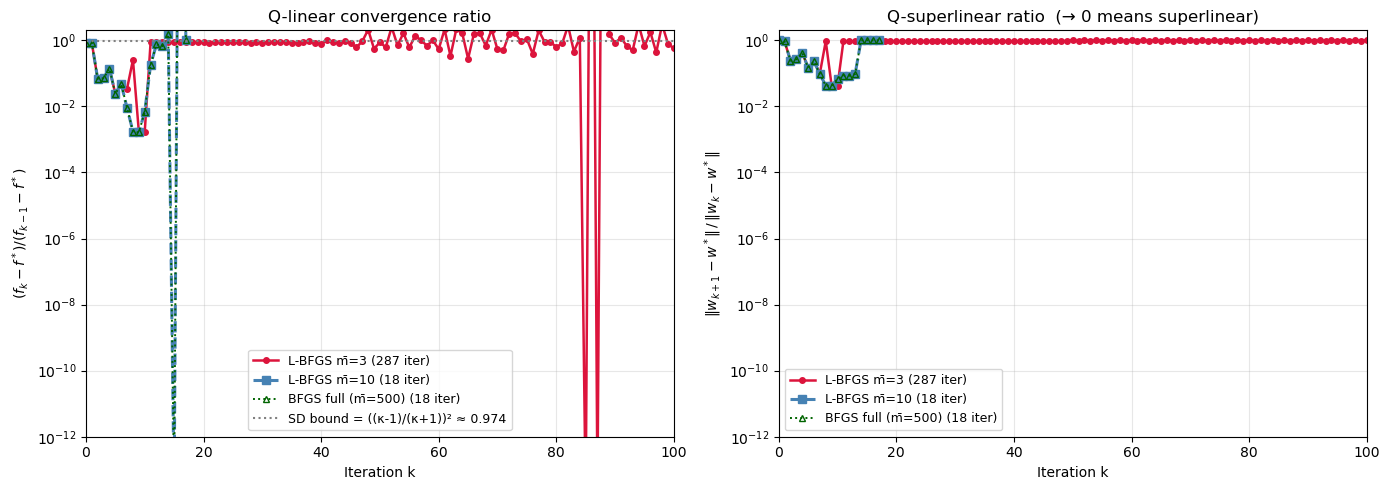
\includegraphics[width=0.80\textwidth]{Chapters/images/convergence_ratios_plot.png}
        \caption{Q-linear (left) and Q-superlinear (right) convergence ratios}
    \end{figure}
    
\noindent The two larger memories, $\bar{m} = 10$ and $\bar{m} = 500$, produce
\emph{identical} trajectories and converge in just $18$ iterations. In the
Q-superlinear panel (right) their ratio descends smoothly to about
$10^{-1}$ before reaching the floor: the stored pairs build a stable,
accurate approximation of the inverse Hessian, so every step is
consistently effective---the behaviour expected of the superlinear regime
of Eq.~\eqref{eq:superlin}. The Q-linear panel (left) shows the
characteristic ``saw-tooth'' of exact line search on a quadratic,
alternating ordinary steps (ratio near $1$) with exceptionally effective
ones (the downward spikes), while always remaining below the
steepest-descent bound $r_{\mathrm{SD}} \approx 0.97$---confirming the
linear bound of Eq.~\eqref{eq:linconv} and that L-BFGS converges far faster
than any first-order method.

\noindent The severely limited memory $\bar{m} = 3$ tells a different story. It
follows the same initial descent but cannot sustain it: with too few
stored pairs, the curvature approximation repeatedly degrades, and the algorithm needs $287$ iterations---over fifteen times more---to reach
the same floor. The restart accelerates this case substantially: without it,
$\bar{m} = 3$ still converges but takes $1{,}147$ iterations, so the restart
yields a roughly fourfold speed-up here (its effect on small memories is
examined in detail in Section~\ref{sec:exp_restart}).

\noindent The contrast between $\bar{m} = 3$ and $\bar{m} \ge 10$ illustrates the
key property of L-BFGS: a small memory matches the full-memory method
\emph{exactly}, provided it exceeds the \emph{effective rank} of the
problem. By Lemma~\ref{lemma:singvals}, $XX^T$ has only $n = 12$ non-zero
eigenvalues, so only $n$ Hessian directions carry non-trivial curvature; a
memory of $\bar{m} \gtrsim n$ captures all of them and any further pairs are
redundant. Storing $10$ vectors is therefore as good as storing all
$500$---and dropping below the effective rank, as with $\bar{m} = 3$,
degrades convergence sharply.


% ─────────────────────────────────────────────────────────────
\subsection{Comparison with Steepest Descent and Conjugate Gradient}
\label{sec:exp_baselines}
% ─────────────────────────────────────────────────────────────

\noindent To assess whether the curvature information used by L-BFGS provides a
practical advantage, we compare it with two natural baselines:
\emph{steepest descent} (SD) with exact line search, and the linear
\emph{conjugate gradient} method (CG) applied to the Symmetric Positive Definite system $Hw = Xy$,
where $H$-vector products are computed implicitly as
$Hv = X(X^Tv) + \lambda^2 v$ at the same $O(mn)$ cost per iteration as L-BFGS.
All methods start from $w_0 = 0$ and use the relative stopping rule
of Eq.~\eqref{eq:stop_rel} with $\varepsilon = 10^{-14}$. Two regimes are
considered: well-conditioned ($\lambda = 1$, $\kappa \approx 76$) and
ill-conditioned ($\lambda = 10^{-4}$, $\kappa \approx 7.6 \times 10^{5}$).

\begin{table}[H]
\centering
\caption{Iteration counts and final gradient norms across four methods
  ($m = 500$, $n = 12$, exact line search, $\varepsilon = 10^{-14}$).}
\label{tab:baselines}
\small
\setlength{\tabcolsep}{12pt}
\begin{tabular}{lcccc}
    \toprule
    & \multicolumn{2}{c}{$\lambda = 1$ ($\kappa \approx 76$)}
    & \multicolumn{2}{c}{$\lambda = 10^{-4}$ ($\kappa \approx 7.6\times10^5$)} \\
    \cmidrule(lr){2-3}\cmidrule(lr){4-5}
    \textbf{Method} & iter & $\norm{\nabla f}$ & iter & $\norm{\nabla f}$ \\
    \midrule
    Steepest Descent           & 1447 & $6.14 \times 10^{-13}$ & 1725 & $6.55 \times 10^{-13}$ \\
    Conjugate Gradient         &   15 & $5.47 \times 10^{-15}$ &   15 & $1.90 \times 10^{-14}$ \\
    L-BFGS ($\bar{m} = 10$)    &   19 & $1.47 \times 10^{-10}$ &   31 & $7.37 \times 10^{-11}$ \\
    Full BFGS ($\bar{m} = 500$)&   19 & $1.47 \times 10^{-10}$ &   31 & $7.37 \times 10^{-11}$ \\
    \bottomrule
\end{tabular}
\end{table}

\begin{figure}[H]
    \centering
    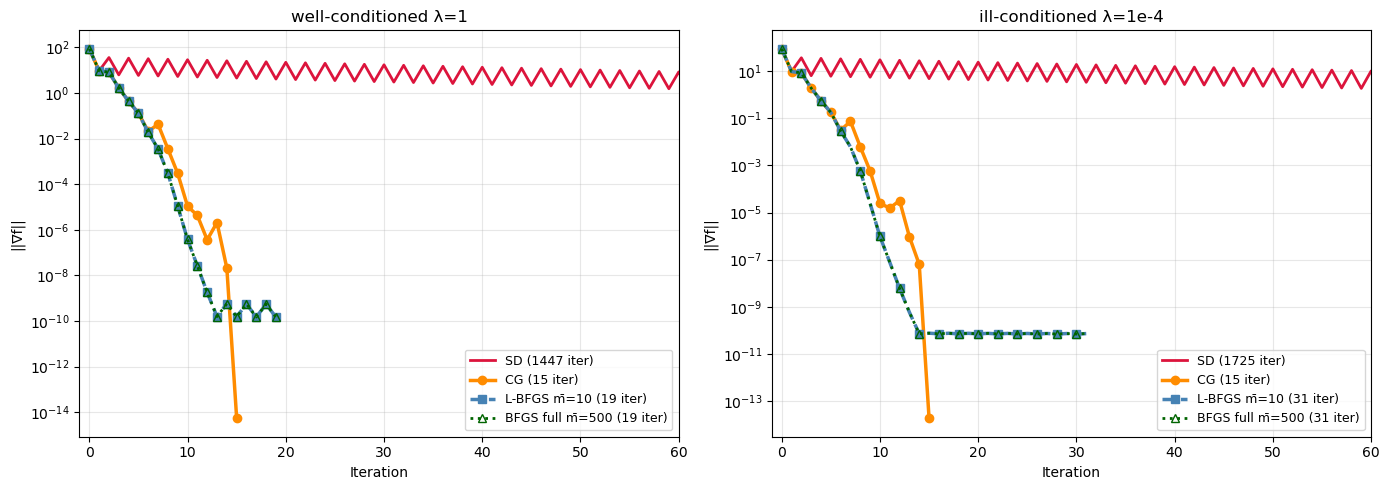
\includegraphics[width=0.80\textwidth]{Chapters/images/comparison_sd_cg.png}
    \caption{Convergence of the four methods ($\norm{\nabla f}$ vs.\
      iteration) in the well-conditioned ($\lambda = 1$, left) and
      ill-conditioned ($\lambda = 10^{-4}$, right) regimes. The $x$-axis is
      truncated at $60$ iterations; SD continues well beyond this range
      (over $1{,}400$ iterations in both cases).}
    \label{fig:baselines}
\end{figure}

\noindent The four methods separate into three performance tiers. Steepest descent
is uncompetitive in both regimes, requiring over $1{,}400$ iterations even
on the well-conditioned problem: using only the gradient, it makes slow
progress along the elongated level sets. L-BFGS with $\bar{m} = 10$ and
full BFGS with $\bar{m} = 500$ produce \emph{identical} trajectories (for
the reason given in Section~\ref{sec:exp_rates}), cutting the iteration
count by nearly two orders of magnitude relative to SD. Conjugate gradient,
however, is faster still, reaching machine precision in just $15$ iterations.

\noindent CG's strong performance is a direct consequence of the problem's algebraic
structure. For SPD systems, CG terminates in a number of iterations equal
to the number of \emph{distinct} eigenvalues of $H$, not its dimension $m$.
As noted in Section~\ref{sec:exp_rates}, $XX^T$ has only $n = 12$ non-zero
eigenvalues (Lemma~\ref{lemma:singvals}); the spectrum of
$H = XX^T + \lambda^2 I$ therefore consists of just $n + 1 = 13$ distinct
values---the $12$ shifted singular values plus $\lambda^2$ with multiplicity
$m - n$. CG resolves this clustered spectrum in roughly $n$ steps regardless
of $\kappa$, which is why it takes $15$ iterations in both regimes.

\noindent Two further effects deserve note. First, conditioning affects L-BFGS but
not CG: raising $\kappa$ from $76$ to $7.6 \times 10^{5}$ increases the
L-BFGS iteration count from $19$ to $31$, while CG stays at $15$. CG's
finite-termination property is immune to $\kappa$, whereas L-BFGS, as a
general quasi-Newton method, is mildly sensitive to it---though far less so
than SD, whose count also grows with $\kappa$ ($1447 \to 1725$). Second, CG
reaches a higher final accuracy ($10^{-14}$--$10^{-15}$ vs.\
$10^{-10}$--$10^{-11}$ for L-BFGS), a consequence of its exact-arithmetic
optimality on quadratics.

\noindent The takeaway is not that L-BFGS is inferior, but that CG wins here precisely
because our problem meets its two ideal assumptions at once: it is
\emph{quadratic} and has a \emph{low-rank, clustered spectrum}. Neither
holds in general---on non-quadratic objectives the conjugacy machinery
breaks down, and on problems with non-clustered spectra CG loses its fast
termination. L-BFGS degrades gracefully in both cases, making it the more
robust choice for the broader class of problems where that structure is
absent.

% ─────────────────────────────────────────────────────────────
\subsection{Alignment with the Newton Direction}
\label{sec:exp_newton}
% ─────────────────────────────────────────────────────────────

\noindent While the previous experiments \emph{observed} superlinear convergence,
this one identifies its \emph{cause}. As anticipated in
Section~\ref{sec:convergence}, Nocedal and
Wright~\cite[Thm.~8.6]{nocedal2006numerical} attribute the superlinear rate
of BFGS to the search direction $p_k = -H_k \nabla f_k$ becoming an
increasingly accurate approximation of the Newton direction
$p_k^{\mathrm{N}} = -H^{-1}\nabla f_k$. We test this directly by measuring
the alignment defect $1 - \cos\theta_k$ between the two directions, using a
cached Cholesky factorisation of $H$ as a measurement oracle. Although this
factorisation costs $O(m^3)$, it is used \emph{only} to compute the
reference Newton direction and is \emph{not} part of the L-BFGS algorithm,
which remains $O(mn + m\bar{m})$ per iteration. To keep the angle
measurement clean, this instrumental variant runs without the
curvature-based restart, so that each trajectory reflects a single,
uninterrupted curvature approximation.

\begin{table}[H]
\centering
\caption{Alignment defect $1 - \cos\theta_k$ at the last \emph{clean}
  iteration (before $\norm{\nabla f}$ reaches the noise floor
  $10^{-9}$).}
\label{tab:newton_angle}
\small
\setlength{\tabcolsep}{12pt}
\begin{tabular}{rcc}
    \toprule
    $\bar{m}$ & \textbf{Clean iterations}
              & \textbf{Final} $1 - \cos\theta_k$ \\
    \midrule
    3        & 40 & $2.83 \times 10^{-1}$ \\
    10, 500  & 13 & $3.53 \times 10^{-3}$ \\
    \bottomrule
\end{tabular}
\end{table}

\noindent The results confirm the mechanism. For $\bar{m} \ge 10$ the defect falls
by two orders of magnitude, reaching $\sim 3.5 \times 10^{-3}$: the L-BFGS
direction becomes nearly indistinguishable from the Newton step, which is
exactly what drives the superlinear regime seen in
Section~\ref{sec:exp_rates}. For $\bar{m} = 3$ the defect stalls at
$\sim 2.8 \times 10^{-1}$ and never improves: with too few stored pairs,
$H_k$ cannot approximate $H^{-1}$ closely enough to recover the Newton
direction. This is the direct cause of its linear-only, much slower
convergence---the $287$ iterations of Section~\ref{sec:exp_rates} are the
price of a search direction that stays misaligned with Newton's. The series
are truncated once $\norm{\nabla f}$ falls below $10^{-9}$, below which both
directions are computed on numerical noise.

\noindent This experiment closes the theoretical loop of
Section~\ref{sec:convergence}: the superlinear convergence of large-memory
BFGS, the linear-only convergence of severely limited L-BFGS, and the
iteration counts of Sections~\ref{sec:exp_rates}
and~\ref{sec:exp_baselines} are all manifestations of the same underlying
mechanism---the quality of the curvature approximation built by the
two-loop recursion.

%% TODO: insert (1 - cos theta_k) vs iter plot, with floor masked

% ═════════════════════════════════════════════════════════════
\section{Algorithmic Design Choices}
\label{sec:exp_design}
% ═════════════════════════════════════════════════════════════

\noindent Each experiment in this section isolates a single design decision in our
L-BFGS implementation and quantifies its impact on convergence. Together,
these experiments justify the default configuration used in the remainder
of the chapter (\texttt{line\_search='exact'}, $\bar{m} = 10$,
\texttt{h0\_scaling='bb1'}, \texttt{use\_restart=True}, $\xi = 0.2$).


% ─────────────────────────────────────────────────────────────
\subsection{Exact Line Search vs.\ Strong Wolfe Line Search}
\label{sec:exp_exact_vs_wolfe}
% ─────────────────────────────────────────────────────────────

\noindent We compare the two line-search strategies at a tight relative tolerance
$\varepsilon = 10^{-14}$, using the standard Wolfe constants
$(c_1, c_2) = (10^{-4}, 0.9)$ recommended by Nocedal and
Wright~\cite[Sec.~3.1]{nocedal2006numerical} for quasi-Newton methods.

\begin{table}[H]
\centering
\caption{Comparison of line-search strategies
  ($m = 500$, $n = 12$, $\lambda = 0.5$, $\bar{m} = 10$,
  $\varepsilon = 10^{-14}$).}
\label{tab:ls_comparison}
\small
\setlength{\tabcolsep}{10pt}
\begin{tabular}{lcccc}
    \toprule
    \textbf{Line Search} & \textbf{Iterations} & $\norm{w - w^*}$
      & \textbf{Time (s)} & \textbf{Stop reason} \\
    \midrule
    Exact   & 18  & $5.44 \times 10^{-12}$ & 0.001 & stagnation \\
    Wolfe ($c_1=10^{-4}, c_2=0.9$) & 599 & $5.21 \times 10^{-8}$ & 0.023 & stagnation \\
    \bottomrule
\end{tabular}
\end{table}

\noindent Exact LS achieves nearly four orders of magnitude higher accuracy
($5.4 \times 10^{-12}$ vs.\ $5.2 \times 10^{-8}$) in only $18$ iterations,
against the $599$ that Wolfe needs before stalling. Its closed-form
minimiser, Eq.~\eqref{eq:exact_alpha_expanded}, exploits the quadratic
structure perfectly at the cost of a single matrix-vector product
$X^T p_k \in O(mn)$.

\noindent The Wolfe variant does not diverge but \emph{stalls}: after roughly the
first $100$ iterations the step length stabilises around
$\alpha \approx 0.07$, too large to trigger the stagnation safeguard but too
small for the curvature condition to extract further progress. The cubic
interpolation inside the bracketing-and-zoom loop loses accuracy once
$\norm{\nabla f} \lesssim 10^{-5}$, the working precision of the line search
itself, and the run eventually stops on stagnation at $599$ iterations.

\noindent An important caveat is that the Wolfe defaults
$(c_1, c_2) = (10^{-4}, 0.9)$ are the standard recommendation for
\emph{non-quadratic} quasi-Newton problems. The next experiment shows that
this default is inappropriate for our quadratic structure: with a stricter
$c_2$, Wolfe LS becomes competitive again.

%% TODO: insert convergence plot (Figure: Exact vs Wolfe, ||grad|| and f vs iter)


% ─────────────────────────────────────────────────────────────
\subsection{Sensitivity to the Wolfe Constants $c_1, c_2$}
\label{sec:exp_wolfe_constants}
% ─────────────────────────────────────────────────────────────

\noindent Building on the previous experiment, we test whether the poor performance of
Wolfe LS is intrinsic or a side effect of the standard $c_2 = 0.9$. We
sweep $c_1 \in \{10^{-4}, 10^{-3}, 10^{-2}\}$ and $c_2 \in \{0.1, \dots, 0.9\}$, recording iterations and final accuracy.

\begin{table}[H]
\centering
\caption{Effect of the Wolfe constants on convergence
  ($m = 500$, $n = 12$, $\lambda = 0.5$, $\bar{m} = 10$,
  $\varepsilon = 10^{-14}$). The three $c_1$ columns are identical,
  confirming that $c_1$ has no effect.}
\label{tab:wolfe_sweep}
\small
\setlength{\tabcolsep}{12pt}
\begin{tabular}{ccccc}
    \toprule
    & \multicolumn{3}{c}{\textbf{Iterations} (by $c_1$)} & \\
    \cmidrule(lr){2-4}
    $c_2$ & $10^{-4}$ & $10^{-3}$ & $10^{-2}$ & $\norm{w - w^*}$ \\
    \midrule
    0.1 & 613 & 613 & 613 & $6.54 \times 10^{-8}$ \\
    0.3 & 26  & 26  & 26  & $1.27 \times 10^{-9}$ \\
    0.5 & 25  & 25  & 25  & $1.88 \times 10^{-9}$ \\
    0.7 & 31  & 31  & 31  & $2.11 \times 10^{-9}$ \\
    0.9 & 599 & 599 & 599 & $5.21 \times 10^{-8}$ \\
    \bottomrule
\end{tabular}
\end{table}

\noindent Two observations stand out. First, $c_1$ has \emph{no} effect: all three
values produce identical iteration counts and accuracies. The Armijo
condition is loose enough to be automatically satisfied at the
curvature-determined trial step, so $c_1$ is structurally inactive here.

\noindent Second, and more interestingly, the dependence on $c_2$ is
\emph{non-monotone}: Wolfe LS performs well across a \emph{broad} interior
range and fails only at the two extremes. For $c_2 \in [0.2, 0.8]$ it
converges in roughly $22$--$34$ iterations---competitive with exact LS
($18$)---whereas both $c_2 = 0.1$ and $c_2 = 0.9$ collapse to $\sim 600$
iterations. The two failures have opposite causes. A large $c_2 = 0.9$ makes
the curvature condition too permissive: it accepts steps that barely reduce
the directional derivative, yielding poor curvature pairs and slow progress.
A small $c_2 = 0.1$ makes it too restrictive: the line search struggles to
locate a step tight enough to satisfy it, and the cubic interpolation
stalls before doing so. Only an intermediate $c_2$ balances the two.

\noindent This experiment reframes the conclusion of
Section~\ref{sec:exp_exact_vs_wolfe}: the apparent ``Wolfe failure'' was
caused entirely by the default $c_2 = 0.9$ landing on a bad extreme. With an
intermediate value such as $c_2 = 0.5$, Wolfe LS converges in $25$
iterations---competitive with, though still slightly slower than, exact LS
at $18$ iterations.

%% TODO: insert convergence plot (||grad|| vs iter, colour = c2, linestyle = c1)


% ─────────────────────────────────────────────────────────────
\subsection{Effect of the Memory Parameter $\bar{m}$}
\label{sec:exp_memory}
% ─────────────────────────────────────────────────────────────

\noindent We vary $\bar{m} \in \{3, 5, 10, 20, 40\}$ using exact line search at the
tight tolerance $\varepsilon = 10^{-14}$, with the curvature-based restart
enabled (as in the default configuration).

\begin{table}[H]
\centering
\caption{Effect of memory size $\bar{m}$ on L-BFGS convergence
  ($m = 500$, $n = 12$, $\lambda = 0.5$, exact LS, restart enabled,
  $\varepsilon = 10^{-14}$).}
\label{tab:memory_effect}
\small
\setlength{\tabcolsep}{12pt}
\begin{tabular}{rcc}
    \toprule
    $\bar{m}$ & \textbf{Iterations} & $\norm{w - w^*}$ \\
    \midrule
    3   & 287 & $9.43 \times 10^{-11}$ \\
    5   & 605 & $2.76 \times 10^{-10}$ \\
    10  & 18  & $5.44 \times 10^{-12}$ \\
    20  & 18  & $5.44 \times 10^{-12}$ \\
    40  & 18  & $5.44 \times 10^{-12}$ \\
    \bottomrule
\end{tabular}
\end{table}

\begin{figure}[H]
    \centering
    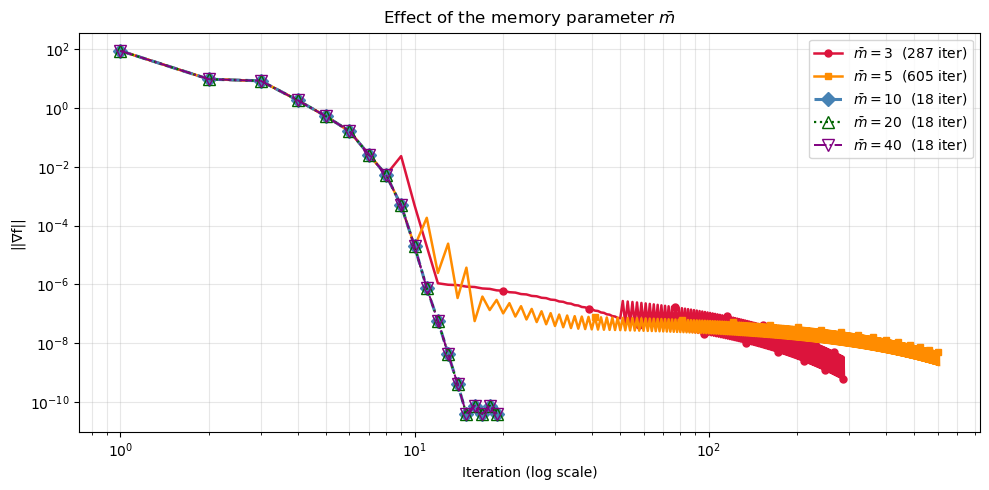
\includegraphics[width=0.70\textwidth]{Chapters/images/memory_effect.png}
    \caption{Gradient-norm convergence for $\bar{m} \in \{3, 5, 10, 20, 40\}$
  (log--log scale, iteration counts in the legend). The curves for
  $\bar{m} \ge 10$ overlap and reach the floor in $18$ iterations. Note the
  non-monotonicity: $\bar{m} = 5$ (orange) lies \emph{above} $\bar{m} = 3$
  (red), taking more than twice as many iterations despite using more
  memory.}
    \label{fig:memory_effect}
\end{figure}

\noindent From $\bar{m} = 10$ onwards the iteration count saturates at $18$ and the
accuracy plateaus at $\norm{w - w^*} \approx 5.4 \times 10^{-12}$. This is the same rank-saturation effect established in
Section~\ref{sec:exp_rates}: a memory of $\bar{m} \gtrsim n = 12$ captures
all the non-trivial curvature directions, so $\bar{m} = 10$, $20$, and $40$
are indistinguishable.

\noindent More striking is the \emph{non-monotone} behaviour at small $\bar{m}$:
$\bar{m} = 3$ takes $287$ iterations, yet $\bar{m} = 5$---with \emph{more}
memory---takes $605$, more than twice as many. This is the documented
non-monotone dependence of L-BFGS on memory
size~\cite[Sec.~9.1]{nocedal2006numerical}: for certain $\bar{m}$ below the
effective rank $n = 12$, the stored curvature pairs interact unfavourably
with the true Hessian spectrum, slowing convergence without affecting the
final accuracy. Adding memory in this regime is no guarantee of faster
convergence, since a larger but still-deficient set of pairs can distort the
search direction more than a smaller one. The practical recommendation is
therefore to set $\bar{m} \gtrsim n$, comfortably above this irregular
regime.

\noindent The small-memory configurations are also where the curvature-based
restart has its strongest effect. At the default $\bar{m} = 10$ the restart
is dormant (it changes nothing), but at $\bar{m} = 3$ it speeds up
convergence appreciably---from $1{,}147$ to $287$ iterations at
$\lambda = 0.5$. Its effect in this regime is, however, not uniformly
beneficial across conditioning; we return to this in
Section~\ref{sec:exp_restart}.

%% TODO: insert plot (||grad|| vs iter on log-x scale, with iter counts in legend)


% ─────────────────────────────────────────────────────────────
\subsection{Effect of the Regularization Parameter $\lambda$}
\label{sec:exp_lambda}
% ─────────────────────────────────────────────────────────────

\noindent We study convergence across five regularization regimes. Recall from
Eq.~\eqref{eq:condition} that $\kappa(\Xhat)$ scales as $O(1/\lambda)$ for
small $\lambda$: weak regularization produces an ill-conditioned, elongated
landscape, while large $\lambda$ drives $\kappa(\Xhat) \to 1$, making the
problem nearly spherical.

\begin{table}[H]
\centering
\caption{Effect of $\lambda$ on condition number and convergence
  ($m = 500$, $n = 12$, exact LS, $\bar{m} = 10$, $\varepsilon = 10^{-14}$).}
\label{tab:lambda_effect}
\small
\setlength{\tabcolsep}{12pt}
\begin{tabular}{lcccc}
    \toprule
    $\lambda$ & $\kappa(\Xhat)$ & \textbf{Iter}
      & $\norm{w - w^*}$ & $t_{\mathrm{LBFGS}}$ (ms) \\
    \midrule
    $10^{-4}$ & $7.6 \times 10^{5}$ & 31 & $1.11 \times 10^{-5}$  & 1.23 \\
    $10^{-2}$ & $7.6 \times 10^{3}$ & 15 & $1.11 \times 10^{-9}$  & 0.69 \\
    $1$       & $75.8$              & 19 & $1.81 \times 10^{-11}$ & 1.01 \\
    $10^{2}$  & $1.3$               &  6 & $3.26 \times 10^{-18}$ & 0.59 \\
    $10^{4}$  & $1.0$               &  3 & $3.99 \times 10^{-22}$ & 0.09 \\
    \bottomrule
\end{tabular}
\end{table}

% \begin{figure}[H]
%     \centering
%     \includegraphics[width=0.75\textwidth]{Chapters/images/lambda_effect_plot.png}
%     \caption{Gradient-norm convergence for five values of $\lambda$.
%       Smaller $\lambda$ (higher $\kappa$) yields a shallower slope; the
%       near-spherical cases $\lambda \ge 10^2$ converge in $3$--$6$ steps.}
%     \label{fig:lambda_effect}
% \end{figure}


\noindent Three observations emerge. First, the iteration count stays small and only
weakly dependent on conditioning: it ranges from $15$ to $31$ across the
three ill- to moderately-conditioned regimes ($\kappa$ from $76$ to
$7.6 \times 10^{5}$), without growing monotonically with $\kappa$. This
confirms that L-BFGS with exact LS converges in $O(n)$ iterations largely
independent of $\kappa$, consistent with the conjugate-direction
interpretation of memoryless BFGS \cite[Sec.~9.1]{nocedal2006numerical} and
with the rank-$12$ structure of $XX^T$ (Lemma~\ref{lemma:singvals}).

\noindent Second, although the iteration count stays low, \emph{final accuracy
degrades sharply with $\kappa$}: from $4 \times 10^{-22}$ at
$\lambda = 10^{4}$ to $1.1 \times 10^{-5}$ at $\lambda = 10^{-4}$. This is
not a failure of the algorithm but the intrinsic floating-point floor of the
normal-equations formulation: forming $XX^T$ squares the condition number
(Eq.~\eqref{eq:Xhat_gram}), so the attainable error is bounded below by
roughly $\kappa^2 \cdot \varepsilon_{\mathrm{mach}}$. At $\lambda = 10^{-4}$
this gives ${\sim}10^{-4}$, consistent with the observed
$1.1 \times 10^{-5}$.

\noindent Third, in the regime $\lambda \gg \sigma_{\max}(X)$ the regularisation term
dominates, $H \approx \lambda^2 I$, and L-BFGS reduces to scaled gradient
descent on a near-spherical problem, converging in $3$--$6$ iterations.
Across all regimes L-BFGS solves the problem in about $1$\,ms.
Section~\ref{sec:exp_cost} examines how this cost scales with $m$.

\noindent Finally, this experiment clarifies why we adopt $\lambda = 0.5$ as the
default for the rest of the chapter. The parameter $\lambda$ is not an
algorithmic knob but part of the problem definition: it sets the
regularisation strength, and hence the trade-off between fitting the data
and controlling $\norm{w}$. Although large $\lambda$ makes the problem
numerically trivial (the case $\lambda = 10^4$ converges in $3$ iterations
to machine precision), the resulting solution is dominated by the penalty
term $\lambda^2\norm{w}^2$ and is essentially $w \approx 0$, ignoring the
data entirely. The value $\lambda = 0.5$ instead yields a moderately
ill-conditioned instance ($\kappa \approx 151$) that is representative of
realistic regularisation and exercises the algorithm in its non-trivial
regime---neither so well-conditioned that convergence is immediate, nor so
ill-conditioned that the problem becomes numerically unsolvable.

%% TODO: insert plot (||grad|| vs iter for the 5 lambda values)


% ─────────────────────────────────────────────────────────────
\subsection{$H_0$ Scaling Strategies}
\label{sec:exp_h0}
% ─────────────────────────────────────────────────────────────

\noindent We compare the three strategies introduced in
Section~\ref{sec:h0_scaling} for the initial Hessian approximation
$H_k^0 = \gamma_k I$ used in the two-loop recursion: the Nocedal default
(BB2, Eq.~\eqref{eq:gamma_nocedal}), the Barzilai--Borwein companion
(BB1, Eq.~\eqref{eq:gamma_bb1}), and the safeguarded variant. To show that the comparison does not depend on
the restart, we run each strategy both with and without it, in both
conditioning regimes.

\begin{table}[H]
\centering
\caption{Effect of $H_0$ scaling on L-BFGS convergence, with and without the
  curvature-based restart ($m = 500$, $n = 12$, exact LS, $\bar{m} = 10$,
  $\varepsilon = 10^{-14}$).}
\label{tab:h0_scaling}
\small
\setlength{\tabcolsep}{9pt}
\begin{tabular}{llcccc}
    \toprule
    & & \multicolumn{2}{c}{\emph{Well-cond.} ($\lambda = 1$, $\kappa \approx 76$)}
      & \multicolumn{2}{c}{\emph{Ill-cond.} ($\lambda = 10^{-2}$, $\kappa \approx 7.6\times10^3$)} \\
    \cmidrule(lr){3-4}\cmidrule(lr){5-6}
    \textbf{Strategy} & \textbf{Restart} & iter & $\norm{w - w^*}$
                                         & iter & $\norm{w - w^*}$ \\
    \midrule
    \texttt{nocedal}     & off & 38 & $3.82\times10^{-12}$ & 29 & $1.11\times10^{-9}$ \\
    \texttt{nocedal}     & on  & 38 & $3.82\times10^{-12}$ & 29 & $1.11\times10^{-9}$ \\
    \texttt{bb1}         & off & 19 & $1.81\times10^{-11}$ & 15 & $1.11\times10^{-9}$ \\
    \texttt{bb1}         & on  & 19 & $1.81\times10^{-11}$ & 15 & $1.11\times10^{-9}$ \\
    \texttt{safeguarded} & off & 38 & $3.82\times10^{-12}$ & 29 & $1.11\times10^{-9}$ \\
    \texttt{safeguarded} & on  & 38 & $3.82\times10^{-12}$ & 29 & $1.11\times10^{-9}$ \\
    \bottomrule
\end{tabular}
\end{table}

\noindent Two clear results emerge. First, \texttt{bb1} converges in roughly
\emph{half} the iterations of the other two strategies---$19$ vs.\ $38$ in
the well-conditioned regime, $15$ vs.\ $29$ in the ill-conditioned one---and
this gap is \emph{identical with and without the restart}, confirming that
it is a genuine property of the scaling rule rather than an interaction with
the restart. The two BB formulas are related by the Cauchy--Schwarz
inequality, which gives $\gamma^{\mathrm{BB1}} \ge \gamma^{\mathrm{N}}$: the
larger initial scale of \texttt{bb1} produces more effective early steps on
this problem, at the cost of a marginally higher final residual
($1.8 \times 10^{-11}$ vs.\ $3.8 \times 10^{-12}$, both at the floor). This
advantage is exactly what led the grid search to select \texttt{bb1} as the
default.

\noindent Second, \texttt{nocedal} and \texttt{safeguarded} produce
\emph{identical} results to the last digit. The safeguard clips $\gamma$
into a safe interval to prevent it from exploding near the solution (where
$y^Ty \to 0$), but on this well-behaved quadratic $\gamma$ never approaches
the clipping bounds, so the safeguard never activates. It is thus free
insurance---inert here, but a cheap guarantee of robustness on problems
where $\gamma$ might otherwise degenerate.

%% TODO: insert convergence plot (3 strategies, two regimes, distinguishable styles)


% ─────────────────────────────────────────────────────────────
\subsection{Curvature-Based Restart}
\label{sec:exp_restart}
% ─────────────────────────────────────────────────────────────

\noindent The curvature-based restart of Liu and
Nocedal~\cite[Sec.~4]{liu1989limited} clears the L-BFGS memory whenever the
curvature ratio $\gamma_k = (s^Ty)/(y^Ty)$ drops by more than a factor
$\xi$ relative to the previous iteration (Eq.~\eqref{eq:restart_cond}),
signalling entry into a region of qualitatively different curvature. We test
it against a no-restart control at two memory sizes: the default
$\bar{m} = 10$ and the severely limited $\bar{m} = 3$, in both conditioning
regimes.

\begin{table}[H]
\centering
\caption{Effect of the curvature-based restart ($\xi = 0.20$) at two memory
  sizes ($m = 500$, $n = 12$, exact LS, \texttt{bb1},
  $\varepsilon = 10^{-14}$).}
\label{tab:restart_effect}
\small
\setlength{\tabcolsep}{9pt}
\begin{tabular}{llcccc}
    \toprule
    & & \multicolumn{2}{c}{\emph{Well-cond.} ($\lambda = 1$)}
      & \multicolumn{2}{c}{\emph{Ill-cond.} ($\lambda = 10^{-2}$)} \\
    \cmidrule(lr){3-4}\cmidrule(lr){5-6}
    $\bar{m}$ & \textbf{Restart} & iter & n\_memory\_clears & iter & n\_memory\_clears \\
    \midrule
    10 & off          & 19  & 1 & 15  & 1 \\
    10 & $\xi = 0.20$  & 19  & 1 & 15  & 1 \\
    \midrule
    3  & off          & 897 & 1 & 332 & 1 \\
    3  & $\xi = 0.20$  & 399 & 3 & 848 & 3 \\
    \bottomrule
\end{tabular}
\end{table}

\noindent The two memory sizes tell opposite stories. With the default
$\bar{m} = 10$ the restart is \emph{dormant}: enabling it leaves the
iteration count unchanged in both regimes ($19$ and $15$). The single
memory clear counted in these runs is not the $\xi$-test at all, but the
negative-curvature reset triggered when $y^Ts$ becomes negligibly small near
the floor (cf.\ Section~\ref{sec:restart}). A sweep over
$\xi \in \{0.05, 0.10, 0.20, 0.40, 0.70\}$ confirms this: all five
thresholds give identical results ($15$ iterations), so the $\xi$-test never
fires when the memory is adequate.
% [DATA] sweep xi conferma dormant a m=10

\noindent The reason is structural. The objective is quadratic, so $H$ is constant
and $\gamma_k$ (Eq.~\eqref{eq:gamma_restart}) stays bounded between
$1/\lambda_{\max}(H)$ and $1/\lambda_{\min}(H)$. With $\bar{m} \ge n$ the
curvature approximation is stable throughout, so $\gamma_k$ never drops by
the factor required to trigger a reset. The mechanism is therefore inert at
the default memory size, adding only negligible overhead.

\noindent With the starved $\bar{m} = 3$, by contrast, the $\xi$-test \emph{does}
fire (three resets in each run), and its effect is substantial but
\emph{not uniformly beneficial}. In the well-conditioned regime it more than
halves the iteration count ($897 \to 399$), as clearing the stale,
rank-deficient memory lets the method rebuild a fresher curvature estimate.
In the ill-conditioned regime, however, it makes matters \emph{worse}
($332 \to 848$): here the discarded pairs, though imperfect, still carried
useful low-curvature information, and rebuilding from scratch repeatedly
costs more than it saves. The restart thus trades stale information for
freshness---a trade that pays off only when the stale information is
genuinely harmful.
% [DATA/STORY] m=3: aiuta well (897->399), peggiora ill (332->848); onesto

\noindent For our purposes the conclusion is clear. At the default $\bar{m} = 10$ the
restart is inactive and costless, so we leave it enabled as a no-risk
safeguard: it never interferes when the memory is adequate, and remains
available should a smaller memory be used. Its variable behaviour at
$\bar{m} = 3$ is a further argument for choosing $\bar{m} \gtrsim n$, where the question does not arise.

% ═════════════════════════════════════════════════════════════
\section{Numerical and Computational Scalability}
\label{sec:exp_scalability}
% ═════════════════════════════════════════════════════════════

\noindent The previous sections established the theoretical and algorithmic behaviour
of L-BFGS on the default ML-CUP instance. We now probe two remaining
practical aspects: how robust the method is to the choice of starting
point, what its theoretical computational cost is, and how it scales empirically
with the problem dimensions $n$ and $m$.

% ─────────────────────────────────────────────────────────────
\subsection{Sensitivity to the Initial Iterate $w_0$}
\label{sec:exp_init}
% ─────────────────────────────────────────────────────────────

\noindent As established in Section~\ref{sec:convergence}, L-BFGS converges from any
starting point on a strongly convex quadratic, with a rate depending only
on $\kappa$. We test four starting points spanning four orders of magnitude
in $\norm{w_0 - w^*}$, from $w_0 = 0$ to a point at distance ${\sim}2{,}000$,
plus one deliberately placed very close to the optimum.

\begin{table}[H]
\centering
\caption{Sensitivity to the initial iterate
  ($m = 500$, $n = 12$, $\lambda = 0.5$, $\bar{m} = 10$, exact LS,
  $\varepsilon = 10^{-14}$).}
\label{tab:init_sensitivity}
\small
\setlength{\tabcolsep}{12pt}
\begin{tabular}{lrcc}
    \toprule
    \textbf{Initialization} & $\norm{w_0 - w^*}$
      & \textbf{Iter} & $\norm{w - w^*}$ \\
    \midrule
    \texttt{zeros}                & $0.85$               & 18 & $5.44 \times 10^{-12}$ \\
    \texttt{random N(0, 1)}       & $22.0$               & 18 & $1.91 \times 10^{-12}$ \\
    \texttt{random N(0, $100^2$)} & $2.19 \times 10^{3}$ & 15 & $1.13 \times 10^{-12}$ \\
    \texttt{near optimum} ($w^* + 0.01 \cdot \mathcal{N}(0,1)$)
                                  & $0.23$               & 41 & $2.83 \times 10^{-12}$ \\
    \bottomrule
\end{tabular}
\end{table}

\noindent The main result is that the \emph{distance} to the optimum does not
determine the iteration count. The three generic starts converge in
$15$--$18$ iterations even though $\norm{w_0 - w^*}$ ranges over four orders
of magnitude; remarkably, the \emph{farthest} start (\texttt{N(0, $100^2$)},
at distance ${\sim}2{,}200$) converges in the \emph{fewest} iterations
($15$). This is the global linear convergence guarantee of
Eq.~\eqref{eq:linconv} in action: on a strongly convex quadratic the rate
depends only on $\kappa$, not on $w_0$. The slight edge of the far start is
a minor geometric effect---a generic point off the origin produces richer
initial curvature pairs than the structured choice $w_0 = 0$---and it is
precisely this artefact that led the grid search to rank random
initialisations marginally above \texttt{zeros}; we nonetheless fix
$w_0 = 0$ as the canonical neutral default.

\noindent The \texttt{near optimum} start is the apparent exception: despite being
the \emph{closest} ($\norm{w_0 - w^*} = 0.23$), it takes the \emph{most}
iterations ($41$). This does not contradict the global convergence result;
it is an artefact of the \emph{relative} stopping criterion
(Eq.~\eqref{eq:stop_rel}). Starting near $w^*$ gives a small initial
gradient $\norm{\nabla f_0}$, so the absolute threshold
$\varepsilon \cdot \norm{\nabla f_0}$ becomes proportionally tighter, and
more iterations are needed to squeeze out the extra orders of magnitude. The
difficulty lies in the convergence \emph{measure}, not in the problem
itself: the final accuracy ($2.8 \times 10^{-12}$) is the same as the other
starts.


% ─────────────────────────────────────────────────────────────
\subsection{Theoretical Cost, Storage, and Scalability}
\label{sec:exp_cost}
% ─────────────────────────────────────────────────────────────

\noindent The main practical motivation for L-BFGS is its favourable cost compared
with a direct solver. Forming and factorising the normal equations
$(XX^T + \lambda^2 I)\,w = Xy$ with \texttt{numpy.linalg.solve} costs
$O(m^3)$, whereas L-BFGS costs $O\big((mn + m\bar{m})\, n_{\mathrm{iter}}\big)$,
with $n_{\mathrm{iter}}$ governed by the conditioning and effective rank
rather than by $m$. We make this concrete with a FLOP count derived from the
structure of the two-loop recursion (Algorithm~\ref{alg:twoloop}). Per
iteration,
\[
  \text{FLOPs/iter} = \underbrace{(4\bar{m} + 1)\,m}_{\text{two-loop}}
                    + \underbrace{2mn}_{\text{gradient}}
                    + \underbrace{mn + 2m}_{\text{exact LS}}
                    + \underbrace{2m}_{\text{update}},
\]
which is linear in both $m$ and $\bar{m}$, while storage is
$2\bar{m}$ vectors of length $m$ plus $O(m)$ working space. Crucially, the
\emph{total} cost to convergence depends on both this per-iteration work
\emph{and} the iteration count, which combine non-trivially.

\begin{table}[H]
\centering
\caption{Total FLOPs to convergence vs.\ $\bar{m}$
  ($m = 500$, $n = 12$, $\lambda = 0.5$, exact LS, $\varepsilon = 10^{-14}$).
  Iteration counts are those of Table~\ref{tab:memory_effect}.}
\label{tab:total_flops}
\small
\setlength{\tabcolsep}{12pt}
\begin{tabular}{rrrrr}
    \toprule
    $\bar{m}$ & \textbf{Iter} & \textbf{FLOPs/iter}
      & \textbf{Total FLOPs} & \textbf{Storage (MB)} \\
    \midrule
    3   & 287 & $26{,}500$  & $7{,}605{,}500$  & 0.040 \\
    5   & 605 & $30{,}500$  & $18{,}452{,}500$ & 0.056 \\
    10  & 18  & $40{,}500$  & $729{,}000$      & 0.096 \\
    20  & 18  & $60{,}500$  & $1{,}089{,}000$  & 0.176 \\
    40  & 18  & $100{,}500$ & $1{,}809{,}000$  & 0.336 \\
    \bottomrule
\end{tabular}
\end{table}

\noindent The total cost is strongly \emph{non-monotone} in $\bar{m}$, driven entirely
by the iteration count of Section~\ref{sec:exp_memory}. The configuration
$\bar{m} = 5$ requires $18.5$M FLOPs---over $25\times$ more than the optimal
$\bar{m} = 10$ at $0.73$M---and even $\bar{m} = 3$ ($7.6$M) outperforms it,
a direct FLOP-level manifestation of the rank-deficient Hessian structure.
The sweet spot is $\bar{m} = 10$: just above the effective rank, it captures
the relevant curvature with minimal redundancy. Increasing $\bar{m}$ further
only inflates the per-iteration cost without reducing the iteration count,
so the total grows linearly beyond this point. Storage is never a
constraint: even $\bar{m} = 40$ uses only $0.34$\,MB, so $\bar{m}$ should be
chosen for convergence speed alone.

\noindent Returning to the comparison with the direct solver, the FLOP model makes
the asymptotic advantage explicit. At the optimal $\bar{m} = 10$, L-BFGS
needs about $0.73$M FLOPs on the present ML-CUP instance ($m=500$). More
generally, if the iteration count remains roughly constant, the total cost
scales approximately linearly in $m$, since each iteration costs
$O(mn + m\bar{m})$. The direct solver, by contrast, scales as $O(m^3)$. For
the ML-CUP dimensions this gap is already substantial, and it widens by a
further factor of about $m^2$ as the problem size grows, which is precisely
the regime where the limited-memory approach becomes indispensable. We verify this scaling empirically---and confirm the
governing role of the effective rank $n$---in Section~\ref{sec:exp_scaling_nm}.


% ─────────────────────────────────────────────────────────────
\subsection{Empirical Scaling with the Dimensions $n$ and $m$}
\label{sec:exp_scaling_nm}
% ─────────────────────────────────────────────────────────────

\noindent The cost analysis above, like all preceding experiments, is based on the
fixed ML-CUP matrix ($m = 500$, $n = 12$). To verify directly how the method
scales with the problem dimensions---and, in particular, to confirm that the
iteration count is governed by the effective rank $n$ rather than by the
sample size $m$---we run two sweeps on synthetic Gaussian data with
standardised columns. We report only iteration counts (which are
deterministic and noise-free) together with $\kappa(\Xhat)$, computed exactly
from the singular values of $X$; this separates the effect of \emph{dimension}
from that of \emph{conditioning}.

\begin{table}[H]
\centering
\caption{Scaling with the number of features $n$ (fixed $m = 500$, exact LS,
  \texttt{bb1}, $\varepsilon = 10^{-14}$). The saturation memory
  $\bar{m}^*$ is the smallest $\bar{m}$ reaching the iteration plateau.}
\label{tab:scaling_n}
\small
\setlength{\tabcolsep}{12pt}
\begin{tabular}{rrrrr}
    \toprule
    $n$ & $\kappa(\Xhat)$ & \textbf{iter L-BFGS}
        & \textbf{iter CG} & $\bar{m}^*$ \\
    \midrule
    5   & 1.17 & 5  & 5  & 3  \\
    12  & 1.28 & 18 & 12 & 10 \\
    25  & 1.50 & 19 & 18 & 23 \\
    50  & 1.84 & 33 & 25 & 48 \\
    100 & 2.46 & 48 & 36 & 98 \\
    \bottomrule
\end{tabular}
\end{table}

% \begin{figure}[H]
%     \centering
%     \includegraphics[width=0.70\textwidth]{Chapters/images/scaling_n.png}
%     \caption{Scaling with the number of features $n$ at fixed $m = 500$ and
%       nearly constant conditioning ($\kappa$ between $1.2$ and $2.5$). The
%       saturation memory $\bar{m}^*$ (red) tracks the reference line $y = n$
%       almost exactly, confirming that the memory required to reach the
%       iteration plateau is the effective rank; CG terminates in at most $n$
%       steps (orange), and the L-BFGS count (blue) grows in step. All three
%       indicators scale with $n$, not with $m$.}
%     \label{fig:scaling_n}
% \end{figure}

\begin{table}[H]
\centering
\caption{Scaling with the sample size $m$ (fixed $n = 12$, exact LS,
  \texttt{bb1}, $\varepsilon = 10^{-14}$).}
\label{tab:scaling_m}
\small
\setlength{\tabcolsep}{12pt}
\begin{tabular}{rrrr}
    \toprule
    $m$ & $\kappa(\Xhat)$ & \textbf{iter L-BFGS} & \textbf{iter CG} \\
    \midrule
    200  & 1.45 & 21 & 12 \\
    500  & 1.28 & 18 & 12 \\
    2000 & 1.15 & 14 & 11 \\
    8000 & 1.06 & 10 &  9 \\
    \bottomrule
\end{tabular}
\end{table}

\noindent The two sweeps confirm the central structural claim of this chapter: the
convergence of both methods is governed by the effective rank $n$, not by the
ambient sample size $m$. As $n$ grows (Table~\ref{tab:scaling_n}), at nearly
constant conditioning, all three indicators scale with $n$. Conjugate
gradient terminates in almost exactly $n$ iterations---$5, 12, 18, 25, 36$
for $n = 5, \dots, 100$---the direct manifestation of its finite-termination
property on the $n+1$ distinct eigenvalues of $H$
(Section~\ref{sec:exp_baselines}). The L-BFGS iteration count grows in step,
and, most tellingly, the saturation memory $\bar{m}^*$ tracks $n$ closely
($3, 10, 23, 48, 98$): the empirical rule $\bar{m} \gtrsim n$ established at
$n = 12$ in Section~\ref{sec:exp_rates} holds across the whole range, with the
threshold shifting in lockstep with the effective rank.

\noindent Varying $m$ at fixed $n$ (Table~\ref{tab:scaling_m}) tells the
complementary story: the iteration count does \emph{not} grow with $m$. It in
fact decreases slightly ($21 \to 10$ for L-BFGS), but this is a conditioning
effect, not a dimension effect---larger Gaussian matrices have better-spread
singular values, so $\kappa$ falls from $1.45$ to $1.06$ over the range, and
fewer iterations are needed. CG likewise stays essentially flat at
${\sim}n$. This is exactly the behaviour predicted by the FLOP model of
Section~\ref{sec:exp_cost}: with the iteration count independent of $m$ and a
per-iteration cost of $O(mn + m\bar{m})$, the total work grows only linearly
in $m$, against the $O(m^3)$ of the direct solver.


% % ─────────────────────────────────────────────────────────────
% \subsection{Numerical Floor as a Function of $\kappa$}
% \label{sec:exp_floor}
% % ─────────────────────────────────────────────────────────────

% \noindent Sections~\ref{sec:exp_lambda} and~\ref{sec:exp_init} suggested that the
% achievable accuracy of L-BFGS is limited by floating-point arithmetic in a
% conditioning-dependent way. We now quantify this directly. Classical
% perturbation theory predicts that for an ill-conditioned linear system the
% relative error in the solution is bounded below by
% \begin{equation}
% \label{eq:wilkinson}
%   \frac{\norm{w - w^*}}{\norm{w^*}} \;\gtrsim\;
%   \kappa(\Xhat)^{2} \cdot \varepsilon_{\mathrm{mach}},
% \end{equation}
% with $\varepsilon_{\mathrm{mach}} \approx 2.22 \times 10^{-16}$ in double
% precision. The exponent $2$ reflects the relation
% $\kappa(H) = \kappa(\Xhat)^{2}$ between the conditioning of $\Xhat$ and that
% of the normal-equations matrix $H = \Xhat^T\Xhat$ (Eq.~\eqref{eq:Xhat_gram}).
% We verify the bound by sweeping $\lambda$ over ten orders of magnitude,
% running L-BFGS with \texttt{tol} $= 0$ for up to $500$ iterations and
% recording the final relative error.

% \begin{table}[H]
% \centering
% \caption{Achieved numerical floor as a function of conditioning
%   ($m = 500$, $n = 12$, exact LS, $\bar{m} = 10$, $\texttt{tol} = 0$).}
% \label{tab:floor}
% \small
% \setlength{\tabcolsep}{12pt} 
% \begin{tabular}{rrrl}
%     \toprule
%     $\lambda$ & $\kappa(\Xhat)$ & \textbf{Iter}
%       & \textbf{Rel.\ error floor} \\
%     \midrule
%     $10^{-6}$ & $7.6 \times 10^{7}$ & 500 & $2.47 \times 10^{-1}$ \\
%     $10^{-5}$ & $7.6 \times 10^{6}$ & 500 & $1.36 \times 10^{-3}$ \\
%     $10^{-4}$ & $7.6 \times 10^{5}$ &  15 & $1.26 \times 10^{-5}$ \\
%     $10^{-3}$ & $7.6 \times 10^{4}$ &  19 & $1.20 \times 10^{-7}$ \\
%     $10^{-2}$ & $7.6 \times 10^{3}$ &  29 & $1.27 \times 10^{-9}$ \\
%     $10^{-1}$ & $7.6 \times 10^{2}$ &  19 & $1.54 \times 10^{-11}$ \\
%     $1$       & $75.8$              &  38 & $4.98 \times 10^{-12}$ \\
%     $10^{1}$  & $7.6$               &  10 & $8.87 \times 10^{-14}$ \\
%     $10^{2}$  & $1.25$              &   6 & $5.85 \times 10^{-16}$ \\
%     $10^{3}$  & $1.0$               &   4 & $4.92 \times 10^{-16}$ \\
%     \bottomrule
% \end{tabular}
% \end{table}

% \noindent The empirical floor follows the bound \eqref{eq:wilkinson} remarkably well.
% From $\kappa = 76$ to $\kappa = 7.6 \times 10^{6}$ the measured curve runs
% parallel to $\kappa^{2}\varepsilon_{\mathrm{mach}}$ in log--log scale with
% an essentially constant ratio of $\sim 0.1$, confirming the slope-$2$
% dependence---a near-perfect quantitative confirmation of classical
% perturbation theory.

% \noindent The bound is structural, not algorithmic: no method operating in double
% precision, iterative or direct, can break this floor, since it is a
% property of the \emph{problem} rather than the \emph{method}. L-BFGS reaches
% it within roughly an order of magnitude of the theoretical limit. For
% $\lambda \le 10^{-5}$ the problem becomes effectively unsolvable in double
% precision: at $\kappa = 7.6 \times 10^{7}$ the predicted floor is
% $\kappa^{2}\varepsilon_{\mathrm{mach}} \approx 1.3$---no meaningful digits
% in $w$---and the $500$-iteration runs at $\lambda \in \{10^{-6}, 10^{-5}\}$
% confirm that no further progress is made. Conversely, at $\kappa \approx 1$
% the floor reaches machine precision $\sim 5 \times 10^{-16}$, where the
% floating-point representation itself is the bottleneck.

% %% TODO: insert plot: empirical floor vs kappa, with kappa*eps and kappa^2*eps reference lines


% ═════════════════════════════════════════════════════════════
\section{Summary}
\label{sec:exp_summary}
% ═════════════════════════════════════════════════════════════

\noindent Our experimental results validate the theoretical predictions of
Section~\ref{sec:convergence} and provide several practical insights into
the design of L-BFGS for this problem class.

\noindent On the \emph{theoretical} side, the empirical convergence ratios confirm
both the global linear bound of Liu and
Nocedal~\cite[Thm.~7.1]{liu1989limited} and the superlinear convergence of
full BFGS~\cite[Thm.~8.6]{nocedal2006numerical}, while the alignment between
the L-BFGS and Newton directions provides a direct mechanistic explanation
of the latter. The comparison against steepest descent and conjugate
gradient positions L-BFGS correctly within the landscape of iterative
methods: although CG outperforms L-BFGS on this specific problem
($15$ vs.\ $19$ iterations) thanks to its finite-termination property on
clustered spectra, L-BFGS would be the method of choice in non-quadratic
settings or on problems with denser Hessian spectra.

\noindent On the \emph{algorithmic} side, exact line search dominates the strong
Wolfe variant for this quadratic problem, converging in $18$ iterations
against the $599$ of the standard Wolfe defaults---though a less extreme
curvature constant ($c_2 = 0.5$ rather than $0.9$) largely closes the gap.
The choice of $H_0$ scaling also matters: the \texttt{bb1} rule converges in
roughly half the iterations of the Nocedal and safeguarded variants, which
is why we adopt it as the default. The most striking finding is the
\emph{non-monotone} dependence on the memory size $\bar{m}$: a larger memory
need not help, with $\bar{m} = 5$ ($605$ iterations) performing worse than
$\bar{m} = 3$ ($287$), while any $\bar{m} \gtrsim n = 12$ saturates at $18$.
This indicates that the optimal memory size sits just above the effective
rank of $XX^T$. The curvature-based restart is dormant at this default
memory size, but becomes active---with a problem-dependent, not uniformly
beneficial, effect---when the memory is starved below the effective rank.

\noindent On the \emph{numerical} side, the per-iteration FLOP model confirms the
favourable cost of L-BFGS: each iteration scales linearly in $m$, against
the $O(m^3)$ of the direct solver, while the iteration count is governed by
the conditioning and effective rank rather than by $m$. This picture is
confirmed by varying the dimensions directly: the iteration count and the
saturation memory $\bar{m}^*$ both track the effective rank $n$, while
holding $n$ fixed and increasing $m$ leaves the iteration count essentially
unchanged. The total cost is
itself non-monotone in $\bar{m}$---mirroring the iteration count---with the
optimal $\bar{m} = 10$ requiring some $25\times$ fewer FLOPs than
$\bar{m} = 5$. Finally, the attainable accuracy tracks the conditioning of
the problem: as $\kappa$ ranges from $1$ to ${\sim}10^{6}$, the final error
degrades from ${\sim}10^{-22}$ to ${\sim}10^{-5}$, consistent with the
floating-point floor $\kappa^2 \varepsilon_{\mathrm{mach}}$ of the
normal-equations formulation.
\clearpage

\chapter{QR Factorization}
% ═════════════════════════════════════════════════════════════
% A2 --- QR Factorization
\label{sec:qr}
% ═════════════════════════════════════════════════════════════

\section{QR Solution of the Regularized Least-Squares Problem}
\label{sec:qr_solution}

\noindent We now turn from the optimization point of view to the direct linear algebra point 
of view. The same regularized least squares problem can be solved without generating 
an iterative sequence of approximations: one factorizes the augmented matrix

\begin{equation}
    A \coloneqq \Xhat =
    \begin{bmatrix}
        X^T \\ \lambda I_m
    \end{bmatrix}
    \in \R^{(n+m)\times m},
    \qquad
    b \coloneqq \yhat =
    \begin{bmatrix}
        y \\ 0
    \end{bmatrix}
    \in \R^{n+m},
\end{equation}

\noindent and then solves the resulting triangular problem. Since $\lambda > 0$, 
Lemma~\ref{lemma:fullrank} shows that $A$ has full column rank. Therefore the 
least squares problem

\begin{equation}
    \min_{w\in\R^m} \norm{Aw-b}
\end{equation}

\noindent has a unique minimizer.

\subsection{Thin QR Factorization}

\noindent For a full column rank matrix $A\in\R^{p\times m}$, with $p=n+m\geq m$, the thin QR 
factorization is

\begin{equation}
\label{eq:thin_qr}
    A = Q_1 R,
    \qquad
    Q_1 \in \R^{p\times m}, \quad Q_1^T Q_1 = I_m,
    \quad
    R \in \R^{m\times m},
\end{equation}

\noindent where $R$ is upper triangular and nonsingular.


\noindent Let $Q_2 \in \R^{p\times n}$ be a matrix whose columns form an orthonormal basis of the orthogonal
complement of $\operatorname{col}(Q_1)$. Then

\begin{equation}
    Q =
    \begin{bmatrix}
    Q_1 & Q_2
    \end{bmatrix}
    \in \R^{p\times p}
\end{equation}

\noindent is an orthogonal matrix:

\begin{equation}
    Q^T Q = Q Q^T = I_p.
\end{equation}

\noindent Therefore,

\begin{equation}
    Q_1^T Q_1 = I_m,
    \qquad
    Q_2^T Q_2 = I_{n},
    \qquad
    Q_2^T Q_1 = 0.
\end{equation}

\noindent Hence,

\begin{equation}
    Q^T A = Q^T Q_1 R =
    \begin{bmatrix}
        R \\ 0
    \end{bmatrix},
    \qquad
    Q^T b =
    \begin{bmatrix}
        Q_1^T b \\ Q_2^T b
    \end{bmatrix} =
    \begin{bmatrix}
        c \\ d
    \end{bmatrix},
    \quad c\in\R^m,\ d\in\R^{n}.
\end{equation}

\noindent Orthogonal transformations preserve the Euclidean norm, hence

\begin{equation}
\label{eq:qr_residual_split}
    \norm{Aw-b}^2
    =
    \norm{Q^T(Aw-b)}^2
    =
    \norm{Rw-c}^2 + \norm{d}^2.
\end{equation}

\noindent Since the term $\norm{d}^2$ is independent of $w$, the minimization problem reduces to
\begin{equation}
\label{eq:qr_triangular_solve}
    \arg\min_{w\in\R^m} \norm{Aw-b}^2
    =
    \arg\min_{w\in\R^m} \norm{Rw-c}^2.
\end{equation}
\noindent Since $R$ is nonsingular, there exists a unique $w$ such that
\begin{equation}
    Rw-c=0,
    \qquad\text{that is,}\qquad
    Rw=c=Q_1^T b.
\end{equation}

\noindent Since $A^T A = (Q_1R)^{T}(Q_1R)$, this is the QR analogue of solving the normal equations. Indeed,

\begin{equation}
\label{eq:qr_normal_equivalence}
    R^T R = A^T A = XX^T + \lambda^2 I_m,
    \qquad
    R^T c = A^T b = Xy.
\end{equation}

\noindent Thus QR and the normal equations define the same solution in exact arithmetic. Numerically, however, 
QR is preferable because it avoids explicitly forming and solving with $A^T A$, whose 
condition number is squared:

\begin{equation}
\label{eq:qr_condition_squaring}
    \kappa_2(A^T A) = \kappa_2(A)^{2}.
\end{equation}

\noindent If $X\neq0$, this distinction is important as $\lambda\to0^+$, since
Eq.~\eqref{eq:condition} gives
$\kappa_2(A)\sim\sigma_{\max}(X)/\lambda$.

\subsection{Algorithmic Structure}

\noindent The QR-based solver can be summarized as follows:

\begin{algorithm}[H]
\caption{QR Solver for the Regularized Least Squares Problem}
\label{alg:qr_solver}
\begin{algorithmic}[1]
    \Require Data matrix $X\in\R^{m\times n}$; response $y\in\R^n$; parameter $\lambda>0$
    \State Form the augmented matrix $A = [X^T;\lambda I_m]$ and vector $b=[y;0]$
    \State Compute a thin QR factorization $A=Q_1R$
    \State Compute $c \gets Q_1^T b$
    \State Solve $Rw=c$ by back-substitution
    \State \Return $w$
\end{algorithmic}
\end{algorithm}

\noindent In practice, the matrix $Q_1$ is not formed explicitly. Forming it would require 
$O((n+m)m)$ storage and applying it as a dense matrix would obscure the sparse and 
structured nature of $A$. Instead, the orthogonal transformations used during the 
factorization are stored in compact form and later applied to $b$.

\subsection{Cost for the QR Solver}
\label{sec:qr_cost_project}
\noindent For a generic dense matrix $A\in\R^{p\times m}$, with $p=n+m\geq m$, computing a thin QR factorization requires

\begin{equation}
    O(pm^2) = O((n+m)m^2)
\end{equation}

\noindent Once the factorization is available, computing the transformed right-hand side $c=Q_1^T b$ requires at most $O(pm)$ additional operations, whereas solving the upper triangular system

\begin{equation}
    Rw=c
\end{equation}

\noindent by back-substitution costs $O(m^2)$.
Therefore, the factorization dominates the overall computational cost. Since $p=n+m$, treating the augmented matrix $A$ as a generic dense matrix gives

\begin{equation}
    O((n+m)m^2) = O(nm^2+m^3),
\end{equation}

\noindent This bound contains a cubic term in $m$.
This is the baseline complexity of the QR solver before exploiting the particular block structure of the augmented matrix. The structured implementation developed in Section~\ref{sec:householder_qr} reduces this cost substantially.


% ═════════════════════════════════════════════════════════════
\section{QR with Householder Reflectors}
\label{sec:householder_qr}
% ═════════════════════════════════════════════════════════════

\noindent Householder reflectors are the standard stable mechanism for computing QR factorizations~\cite{trefethen1997,golub2013}. The implementation stores a normalized reflector vector $u$, so a Householder reflector has the form

\begin{equation}
\label{eq:householder_def}
    H = I - 2uu^T,
    \qquad
    \norm{u}_2=1.
\end{equation}

\noindent Equivalently, for an unnormalized nonzero vector $v$, one may write
$H=I-\tau vv^T$ with $\tau=2/(v^T v)$. In either representation, $H$ is
symmetric and orthogonal:

\begin{equation}
    H^T = H,
    \qquad
    H^T H = I.
\end{equation}

\noindent Given a nonzero vector $z\in\R^\ell$, the reflector is chosen so that all
components below the first one are annihilated. To match the implementation and
avoid overflow or underflow in the norm calculation, define

\begin{equation}
\label{eq:stable_householder_vector}
    s=\norm{z}_\infty,
    \qquad
    \bar z=\frac{z}{s},
    \qquad
    \nu=\norm{\bar z}_2,
    \qquad
    \sigma=\begin{cases}1,&z_1\geq0,\\-1,&z_1<0,
    \end{cases}
\end{equation}

\noindent and then

\begin{equation}
    \alpha=-\sigma s\nu,
    \qquad
    v=\bar z+\sigma\nu e_1,
    \qquad
    u=\frac{v}{\norm{v}_2}.
\end{equation}

\noindent With $H$ as in Eq.~\eqref{eq:householder_def}, this construction gives

\begin{equation}
    Hz = \alpha e_1
    = 
    \begin{bmatrix}
        -\operatorname{sign}(z_1)\norm{z}_2 \\
        0 \\
        \vdots \\
        0
    \end{bmatrix}.
\end{equation}

\noindent Thus the convention is $\operatorname{sign}(0)=1$. The sign choice makes
the first component of $v$ an addition of like-signed quantities, thereby
avoiding subtractive cancellation. If $z=0$, the code returns $u=0$ and
$\alpha=0$ as an identity-reflector sentinel; reflector-application routines
skip this sentinel.

\noindent At step $i$, the current active column is therefore mapped to a vector
whose entries below position $i$ are zero, while its $i$-th entry becomes
$\alpha$.

\subsection{Dense Householder QR}

\noindent The function \texttt{naive\_qr\_solver} applies Householder QR to the
explicit augmented matrix as if it were generic and dense; here \emph{naive}
means that the block structure is ignored, not that the transformation is
unstable. For $A\in\R^{p\times m}$, the factorization proceeds column by
column. At step $k$, one constructs an active reflector
$\widehat H_k\in\R^{(p-k+1)\times(p-k+1)}$ such that

\begin{equation}
    \widehat H_k A_{k:p,k}
    =
    \begin{bmatrix}
        \alpha_k \\ 0 \\ \vdots \\ 0
    \end{bmatrix}.
\end{equation}

\noindent The same active reflector is applied to the whole trailing submatrix
$A_{k:p,k:m}$. Let $H_k=\operatorname{diag}(I_{k-1},\widehat H_k)$ denote
its extension to $\R^p$. After $m$ steps,

\begin{equation}
    H_m\cdots H_2H_1 A =
    \begin{bmatrix}
        R \\ 0
    \end{bmatrix}.
\end{equation}

\noindent Since each Householder reflector is orthogonal, their product is also
orthogonal. Defining

\begin{equation}
    Q^T = H_m \cdots H_2 H_1,
    \qquad
    Q \in \R^{p\times p},
\end{equation}

\noindent we obtain

\begin{equation}
    Q^T A =
    \begin{bmatrix}
        R \\
        0
    \end{bmatrix},
    \quad
    R \in \R^{m\times m},
\end{equation}

\noindent where $R$ is upper triangular. Multiplying by $Q$ gives

\begin{equation}
    A =
    Q
    \begin{bmatrix}
        R \\
        0
    \end{bmatrix}.
\end{equation}

\noindent Let $Q_1 \in \R^{p\times m}$ denote the first $m$ columns of $Q$. Since the remaining rows of the block matrix above are zero, this reduces to the thin QR factorization

\begin{equation}
    A = Q_1 R,
    \qquad
    Q_1^T Q_1 = I_m.
\end{equation}

\noindent The important implementation point is that $Q$ is never formed explicitly.
The dense implementation first stores the normalized reflector vectors and then
applies them to a copy of $b$, in factorization order:

\begin{equation}
    b_{k:p} \leftarrow \widehat H_k b_{k:p}
    =
    b_{k:p} - 2u_k \left(u_k^T b_{k:p}\right).
\end{equation}

\noindent After all $m$ reflectors have been applied, the work vector contains $Q^T b$. Its first
$m$ entries are

\begin{equation}
    c = Q_1^T b,
\end{equation}

\noindent This is the right-hand side of the triangular system $Rw=c$.

\begin{algorithm}[H]
\caption{Compact Dense Householder QR}
\label{alg:householder_dense}
\begin{algorithmic}[1]
    \Require Matrix $A\in\R^{p\times m}$ with $p\geq m$
    \For{$k=1,\ldots,m$}
        \State $z \gets A_{k:p,k}$
        \State $(u,\alpha) \gets \Call{StableHouseholderVector}{z}$ using Eq.~\eqref{eq:stable_householder_vector}
        \If{$u\neq0$}
            \State $A_{k:p,k:m} \gets A_{k:p,k:m} - 2u(u^T A_{k:p,k:m})$
        \EndIf
        \State $A_{kk}\gets\alpha$; \quad $A_{k+1:p,k}\gets0$
        \State Store $u$
    \EndFor
    \State $R \gets \mathrm{triu}(A_{1:m,1:m})$
    \State \Return $R$ and stored reflectors
\end{algorithmic}
\end{algorithm}

\noindent Algorithm~\ref{alg:householder_dense} is the mathematically canonical version. It is 
useful for explaining QR, but for the project matrix it should be specialized as 
described next.

\subsection{Structure-Based Householder QR}
\label{sec:structured_householder}

\noindent The augmented matrix has the special block structure

\begin{equation}
    A = \begin{bmatrix} X^T \\
    \lambda I_m \end{bmatrix}, \qquad b = \begin{bmatrix} y \\
    0 \end{bmatrix}.
\end{equation}

\noindent The order of the rows is irrelevant for the least-squares problem. Indeed, if $P$ is a permutation matrix, then $P$ is orthogonal and therefore

\begin{equation}
    \norm{Aw-b} = \norm{P(Aw-b)}.
\end{equation}

\noindent We can consequently work with the equivalent permuted system

\begin{equation}
    \label{eq:permuted_augmented} \tilde{A} = \begin{bmatrix} \lambda I_m \\ X^T \end{bmatrix}, \qquad \tilde{b} = \begin{bmatrix} 0 \\ y \end{bmatrix}.
\end{equation}

\noindent This ordering is particularly convenient because the first $m$ rows already form an upper triangular matrix,

\begin{equation}
    R_0=\lambda I_m.
\end{equation}

\noindent The function \texttt{qr\_solver\_structure\_based} performs a column sweep
without forming the full $(m+n)\times m$ matrix. Let $Z=X^T$ denote the dense
lower block. At step $k$, it forms only the active block

\begin{equation}
\label{eq:structure_active_block}
    B_k=
    \begin{bmatrix}
        R_{k,k:m}\\
        Z_{:,k:m}
    \end{bmatrix}
    \in\R^{(n+1)\times(m-k+1)}.
\end{equation}

\noindent A normalized reflector $u_k\in\R^{n+1}$ is computed from the first
column of $B_k$. The update

\begin{equation}
    B_k\leftarrow B_k-2u_k(u_k^T B_k)
\end{equation}

\noindent annihilates all $n$ entries of $Z_{:,k}$ at once. Its first row is
written back to $R_{k,k:m}$ and its remaining rows to $Z_{:,k:m}$. Thus the
algorithm stores $m$ reflectors of fixed length $n+1$, rather than the
decreasing reflectors of length $m+n-k+1$ used by dense QR.

\noindent The same reflectors are applied to the permuted right-hand side without
forming $Q$. At step $k$, only the leading coordinate $c_k$ and the current
dense tail $z\in\R^n$ are active:

\begin{equation}
\label{eq:structure_rhs_update}
    q=\begin{bmatrix}c_k\\z\end{bmatrix},
    \qquad
    q\leftarrow q-2u_k(u_k^T q),
    \qquad
    c_k\leftarrow q_1,
    \quad z\leftarrow q_{2:n+1}.
\end{equation}

\noindent After the last update, $c\in\R^m$ is the leading part of
$Q^T\tilde b$ required by the triangular solve. In the current Python work
buffer, these first $m$ components are returned correctly, but the final
transformed tail $z$ is not copied back; consequently, the last $n$ entries
of the returned buffer must not be interpreted as the complete lower part of
$Q^T\tilde b$.

\begin{algorithm}[H]
\caption{Structure-Based Householder QR by Columns}
\label{alg:structure_based_householder}
\begin{algorithmic}[1]
    \Require $X\in\R^{m\times n}$, $y\in\R^n$, $\lambda>0$
    \State $R\gets\lambda I_m$; \quad $Z\gets X^T$
    \For{$k=1,\ldots,m$}
        \State $B\gets[R_{k,k:m};\,Z_{:,k:m}]$
        \State $(u_k,\alpha_k)\gets\Call{StableHouseholderVector}{B_{:,1}}$
        \If{$u_k\neq0$}
            \State $B\gets B-2u_k(u_k^T B)$
        \EndIf
        \State $B_{11}\gets\alpha_k$; \quad $B_{2:n+1,1}\gets0$
        \State $R_{k,k:m}\gets B_{1,:}$; \quad $Z_{:,k:m}\gets B_{2:n+1,:}$
        \State Store $u_k$
    \EndFor
    \State $c\gets0\in\R^m$; \quad $z\gets y$
    \For{$k=1,\ldots,m$}
        \State $q\gets[c_k;\,z]$
        \If{$u_k\neq0$}
            \State $q\gets q-2u_k(u_k^T q)$
        \EndIf
        \State $c_k\gets q_1$; \quad $z\gets q_{2:n+1}$
    \EndFor
    \State $w\gets\Call{BackSubstitution}{R,c}$
    \State \Return $R,w,c$ and the stored reflectors
\end{algorithmic}
\end{algorithm}

\subsection{Two-Dimensional Householder Row Insertion}
\label{sec:row_insertion_householder}

\noindent A second implementation is based on the mathematically valid idea of
inserting the remaining $n$ rows of $X^T$ one at a time.
At iteration $i$, let $x_i^T = [a_1,\ldots,a_m]$ be the new data row and $y_i$ its corresponding right-hand-side entry. We maintain the current upper triangular factor $R_{i-1}$ and the transformed right-hand side $c_{i-1}$.

\noindent Appending the new row gives

\begin{equation}
    \begin{bmatrix}
        R_{i-1} \\
        x_i^T
    \end{bmatrix}
    =
    \begin{bmatrix}
        R_{11} & R_{12} & R_{13} & \cdots & R_{1m} \\
        0      & R_{22} & R_{23} & \cdots & R_{2m} \\
        0      & 0      & R_{33} & \cdots & R_{3m} \\
        \vdots & \vdots & \ddots & \ddots & \vdots \\
        0      & 0      & \cdots & 0      & R_{mm} \\
        a_1    & a_2    & a_3    & \cdots & a_m
    \end{bmatrix}
    \in \R^{(m+1)\times m}.
\end{equation}

\noindent A sequence of $m$ Householder reflectors is then applied to eliminate the entries of the inserted row one at a time, yielding

\begin{equation}
    \begin{bmatrix}
        R_{i-1} \\
        x_i^T
    \end{bmatrix}
    \longrightarrow
    \begin{bmatrix}
        R_i \\
        0
    \end{bmatrix}
    =
    \begin{bmatrix}
        R^{(i)}_{11} & R^{(i)}_{12} & R^{(i)}_{13} & \cdots & R^{(i)}_{1m} \\
        0            & R^{(i)}_{22} & R^{(i)}_{23} & \cdots & R^{(i)}_{2m} \\
        0            & 0            & R^{(i)}_{33} & \cdots & R^{(i)}_{3m} \\
        \vdots       & \vdots       & \ddots       & \ddots & \vdots \\
        0            & 0            & \cdots       & 0      & R^{(i)}_{mm} \\
        0            & 0            & \cdots       & 0      & 0
    \end{bmatrix}.
\end{equation}

\noindent The same orthogonal transformations must be applied to the corresponding right-hand side:

\begin{equation}
    \begin{bmatrix}
        c_{i-1} \\
        y_i
    \end{bmatrix}
    =
    \begin{bmatrix}
        c_1 \\
        c_2 \\
        \vdots \\
        c_m \\
        y_i
    \end{bmatrix}
    \longrightarrow
    \begin{bmatrix}
        c^{(i)}_1 \\
        c^{(i)}_2 \\
        \vdots \\
        c^{(i)}_m \\
        \eta_i
    \end{bmatrix}
    =
    \begin{bmatrix}
        c_i \\
        \eta_i
    \end{bmatrix}.
\end{equation}

\noindent Unlike the inserted row of the matrix, the last component $\eta_i$ of the transformed right-hand side is not generally zero. Since it corresponds to a zero row in the transformed matrix, it is independent of $w$ and therefore does not affect the least-squares minimizer. Consequently, only the updated vector $c_i$ needs to be retained for the subsequent row insertions and for the final triangular solve $R_n w = c_n$. The scalar $\eta_i$ may be discarded unless the final residual norm is also required.

\noindent At step $k$, the current matrix $R$ is already upper triangular and the
previous components $a_1,\ldots,a_{k-1}$ of the inserted row have already
been annihilated. Therefore, in column $k$, the only nonzero entry below the
diagonal is the active element $a_k$.

\noindent For this reason, it is not necessary to build a Householder reflector on the
entire column. It is sufficient to consider only the two entries involved in
the elimination,

\begin{equation}
    z =
    \begin{bmatrix}
        R_{kk} \\
        a_k
    \end{bmatrix}
    \in \R^2.
\end{equation}

\noindent A two-dimensional normalized Householder reflector is then constructed as

\begin{equation}
    H_k^{(i)} = I_2 - 2u u^T,
    \qquad \norm{u}_2=1,
\end{equation}

\noindent and chosen so that

\begin{equation}
    H_k^{(i)}
    \begin{bmatrix}
        R_{kk} \\
        a_k
    \end{bmatrix}
    =
    \begin{bmatrix}
        \rho \\
        0
    \end{bmatrix}.
\end{equation}

\noindent Thus, at each step only the pair $(R_{kk},a_k)$ is needed to determine the
reflector: the diagonal entry is updated to $\rho$, while the corresponding
entry of the inserted row is annihilated.

\noindent The same $2\times2$ reflector must then be applied to the remaining entries
of the two affected rows, so that the transformation is consistent across
the whole trailing part of the matrix:

\begin{equation}
    \begin{bmatrix}
        R_{k,k:m} \\
        a_{k:m}
    \end{bmatrix}
    \leftarrow
    H_k^{(i)}
    \begin{bmatrix}
        R_{k,k:m} \\
        a_{k:m}
    \end{bmatrix}.
\end{equation}

\noindent The corresponding right-hand-side entries are transformed by the same reflector,

\begin{equation}
    \begin{bmatrix}
        c_k \\
        \eta
    \end{bmatrix}
    \leftarrow
    H_k^{(i)}
    \begin{bmatrix}
        c_k \\
        \eta
    \end{bmatrix},
\end{equation}

\noindent Here $\eta$ is initialized as $\eta=y_i$ at the beginning of the insertion of row $x_i^T$.

\noindent After repeating this procedure for $k=1,\ldots,m$, all entries of the inserted row have been annihilated. The row can then be discarded, while the updated $R$ and $c$ contain the effect of the newly inserted data row.

\begin{algorithm}[H]
\caption{Two-Dimensional Householder Row Insertion}
\label{alg:row_insertion_householder}
\begin{algorithmic}[1]
    \Require $X\in\R^{m\times n}$, $y\in\R^n$, $\lambda>0$
    \State $R \gets \lambda I_m$; \quad $c \gets 0\in\R^m$
    \For{$i=1,\ldots,n$}
        \State $a \gets X_{:,i}$; \quad $\eta \gets y_i$
        \For{$k=1,\ldots,m$}
            \State $z \gets [R_{kk},\, a_k]^{T}$
            \State $(u,\rho)\gets\Call{StableHouseholderVector}{z}$
            \State $H\gets I_2-2uu^T$
            \State $[R_{k,k:m};\,a_{k:m}] \gets H [R_{k,k:m};\,a_{k:m}]$
            \State $[c_k;\,\eta] \gets H[c_k;\,\eta]$
            \State Store the reflector record $(k,m+i,u)$
        \EndFor
    \EndFor
    \State Solve $Rw=c$ by back-substitution
    \State \Return $w$
\end{algorithmic}
\end{algorithm}

\subsection{Runtime Scalability}
\label{sec:qr_scalability}

\noindent The column-oriented structure-based method applies one reflector to an
$(n+1)\times(m-k+1)$ block at each step. Its factorization cost is therefore

\begin{equation}
\label{eq:structure_based_qr_cost}
    \sum_{k=1}^{m}O\bigl((n+1)(m-k+1)\bigr)
    =O(nm^2+m^2).
\end{equation}

\noindent Applying the reflectors to the right-hand side costs $O(nm)$ and back
substitution costs $O(m^2)$. The complete structure-based solver thus costs
$O(nm^2+m^2)$. The row-insertion algorithm has the same order:
for each of the $n$ data rows, it applies $m$ transformations to trailing
segments, at a cost

\begin{equation}
    \sum_{i=1}^{n}\sum_{k=1}^{m}O(m-k+1)=O(nm^2),
\end{equation}

\noindent followed by $O(m^2)$ back substitution.

\noindent Combining these bounds with Section~\ref{sec:qr_cost_project} gives

\begin{equation}
\label{eq:qr_scaling_summary}
\begin{aligned}
    T_{\mathrm{dense\ QR}}(m,n) &= O(m^3+nm^2),\\
    T_{\mathrm{structure\text{-}based\ QR}}(m,n) &= O(m^2+nm^2),\\
    T_{\mathrm{row\ insertion}}(m,n) &= O(m^2+nm^2),\\
    T_{\mathrm{normal\ equations}}(m,n) &= O(m^3+nm^2).
\end{aligned}
\end{equation}

\noindent Hence, with the project value $n=12$ fixed, both structured algorithms
are quadratic in $m$, whereas generic dense QR and a dense normal-equations
solve retain a cubic term. The structure-based implementation stores the
triangular factor, a copy of the dense block, and $m$ reflectors of length
$n+1$, for $O(m^2+nm)$ memory. The current row-insertion wrapper also stores
all $nm$ two-dimensional reflector records; disabling that optional storage
would leave only $O(m)$ workspace in addition to $R$.

\noindent The notebook first constructs a single matrix with $4000$ rows by
calling \texttt{build\_augmented\_X} with seed $42$ and jitter $0.01$. The
original $500$ rows are retained as the leading block; each additional row is
sampled as a complete row of $X$ and perturbed by Gaussian noise scaled by the
empirical standard deviation of each column. Taking prefixes of this matrix
produces nested problems with fixed $n=12$,
$m\in\{100,250,500,1000,2000,4000\}$, and $\lambda=0.5$. Data generation is
performed once, outside every timed region. Each entry in
Table~\ref{tab:qr_runtime_scaling} is the arithmetic mean of ten runs, without
a warm-up or randomized execution order.

\begin{table}[H]
\centering
\caption{Internal solver times in milliseconds for the augmented-data runtime
sweep. The normal-equations timer is partial.}
\label{tab:qr_runtime_scaling}
\small
\setlength{\tabcolsep}{5pt}
\begin{tabular}{rrrrr}
    \toprule
    $m$ & \textbf{Normal eq.} & \textbf{Dense QR}
        & \textbf{Structure-based QR} & \textbf{Row insertion}\\
    \midrule
     100 &    0.138 &      5.440 &   3.840 &  12.543\\
     250 &    1.333 &     70.165 &  18.151 &  68.379\\
     500 &    6.235 &    288.259 &  40.001 &  75.609\\
    1000 &   39.286 &   3830.648 &  61.597 & 143.880\\
    2000 &  296.157 &  26490.742 & 157.124 & 314.136\\
    4000 & 1628.571 & 180615.340 & 422.753 & 777.798\\
    \bottomrule
\end{tabular}
\end{table}

\noindent The solver timers still do not have identical scopes. The
normal-equations baseline measures only \texttt{numpy.linalg.solve}, excluding
construction of $XX^T+\lambda^2I_m$, construction of $Xy$, and evaluation of
the objective. In the current code, dense QR starts its timer before building
$A$ and $b$, while structure-based QR starts before building $[0;y]$; both
then include factorization, right-hand-side transformation, and back
substitution. Row insertion includes its fused right-hand-side updates and the
storage of all reflectors. Consequently, the normal-equations column prevents
Table~\ref{tab:qr_runtime_scaling} from being a uniform end-to-end comparison.

\noindent Within the comparable QR timings, at $m=4000$ the structure-based
path takes approximately $0.423$ seconds and row insertion $0.778$ seconds,
versus $180.615$ seconds for dense QR; the structure-based method is therefore
about $427$ times faster than dense QR at this size. On the final doubling from
$m=2000$ to $m=4000$, the dense, structure-based, and row-insertion times
increase by factors of approximately $6.82$, $2.69$, and $2.48$, respectively,
which is consistent with the cubic and quadratic terms in
Eq.~\eqref{eq:qr_scaling_summary}. These six measurements are empirical
evidence, not a proof of asymptotic complexity; moreover, the notebook computes
reference-slope arrays but does not draw them.

\subsection{Algorithmic Stability and the Condition Number}
\label{sec:qr_stability}

\noindent Conditioning is a property of the mathematical problem, whereas
stability is a property of the algorithm used to solve it. For
$A=[X^T;\lambda I_m]$,

\begin{equation}
    A^T A=XX^T+\lambda^2I_m.
\end{equation}

\noindent Since the project has $m>n$, the matrix $XX^T$ has at least $m-n$
zero eigenvalues. Therefore

\begin{equation}
\label{eq:qr_condition_lambda}
    \kappa_2(A)
    =\frac{\sqrt{\sigma_{\max}(X)^{2}+\lambda^2}}{\lambda},
    \qquad \lambda>0.
\end{equation}

\noindent If $X\neq0$, Eq.~\eqref{eq:qr_condition_lambda} behaves as
$\sigma_{\max}(X)/\lambda$ when $\lambda\to0^+$ and tends to $1$ as
$\lambda\to\infty$. Forming the normal equations squares this number, as
shown in Eq.~\eqref{eq:qr_condition_squaring}; this is precisely the
conditioning penalty avoided by Householder QR.

\noindent In the standard floating-point model with machine precision
$\varepsilon_{\mathrm{mach}}$, Householder QR is backward stable: up to
dimension-dependent constants, the computed factors are the exact QR factors
of $A+\Delta A$ with

\begin{equation}
    \frac{\norm{\Delta A}_2}{\norm{A}_2}=O(\varepsilon_{\mathrm{mach}}),
\end{equation}

\noindent and the computed orthogonal factor is orthogonal to working precision.
The resulting forward error still depends on the conditioning and geometry of
the least-squares problem. Accordingly, the notebook uses
$\varepsilon_{\mathrm{mach}}\kappa_2(A)$ for QR and
$\min\{1,\varepsilon_{\mathrm{mach}}\kappa_2(A)^{2}\}$ for normal equations
only as heuristic trend guides. They are not universal error bounds: the
forward condition number of the least-squares solution also depends on the
residual geometry. The notebook additionally plots
$\varepsilon_{\mathrm{mach}}$ as a reference scale for
$\eta_{\mathrm{opt}}$.

\noindent The notebook diagnoses this behavior using an independent thin-SVD
reference. If $X=U\Sigma V^T$, then the Tikhonov solution is

\begin{equation}
\label{eq:qr_svd_reference}
    w_{\mathrm{SVD}}
    =U\operatorname{diag}\!\left(
        \frac{\sigma_i}{\sigma_i^2+\lambda^2}
      \right)V^T y.
\end{equation}

\noindent For a computed solution $w$, the two reported diagnostics are the
relative forward error

\begin{equation}
\label{eq:qr_forward_error}
    e_{\mathrm{fwd}}
    =\frac{\norm{w-w_{\mathrm{SVD}}}_2}{\norm{w_{\mathrm{SVD}}}_2}
\end{equation}

\noindent and, for the augmented residual $r=Aw-b\neq0$, the scaled first-order
optimality residual

\begin{equation}
\label{eq:qr_scaled_optimality}
    \eta_{\mathrm{opt}}
    =\frac{\norm{A^T r}_2}{\norm{A}_2\norm{r}_2}.
\end{equation}

\noindent At an exact least-squares solution $A^T r=0$, so a small
$\eta_{\mathrm{opt}}$ verifies the optimality condition. It does not by itself
guarantee a small forward error when $A$ is severely ill-conditioned; both
diagnostics must therefore be considered together.

\noindent The experiment sweeps $\lambda\in\{10^j:j=-12,\ldots,4\}$. The
current dense solver receives $X$, $y$, and the current value of $\lambda$ at
every iteration, so its augmented system is now rebuilt correctly throughout
the sweep. For normal equations, dense QR, and structure-based QR,
respectively, the relative forward errors at $\lambda=10^{-6}$, where
$\kappa_2(A)\approx7.575\times10^7$, are approximately
$4.04\times10^{-1}$, $6.08\times10^{-14}$, and $1.11\times10^{-9}$. At
$\lambda=10^{-12}$, where
$\kappa_2(A)\approx7.575\times10^{13}$, they are approximately
$1.55\times10^1$, $4.04\times10^{-14}$, and $6.43\times10^{-4}$. At these two
ill-conditioned sample points, both Householder methods are substantially more
accurate than the explicitly formed normal equations, and dense QR has the
smallest forward error. Its near-machine-precision forward error at very small
$\lambda$ is an empirical property of this problem and must not be interpreted
as a universal conditioning-independent guarantee.

\noindent In the same method order, the corresponding
$\eta_{\mathrm{opt}}$ values are $6.63\times10^{-9}$,
$4.89\times10^{-10}$, and $9.03\times10^{-10}$ at $\lambda=10^{-6}$, and
$1.92\times10^{-3}$, $2.01\times10^{-3}$, and $6.64\times10^{-5}$ at
$\lambda=10^{-12}$. The extreme case also illustrates why forward error and
scaled optimality must be read together: dense QR has the smallest forward
error there, whereas structure-based QR has the smallest scaled optimality
residual.

\noindent One execution-state limitation remains in the saved notebook. Although
the row-insertion source has been corrected, the run retained the old imported
function in the active kernel. Its stored row-insertion accuracy and stability
values are therefore obsolete and are excluded from the conclusions above.
The printed scaled-optimality table correctly indexes the stored arrays, and
the condition numbers, SVD reference calculations, normal-equations results,
dense-QR results, and structure-based results are valid and support the
comparison made here.

\clearpage

% \chapter{Comparison: QR vs. L-BFGS}
% % ═════════════════════════════════════════════════════════════
% Comparison: QR vs.\ L-BFGS
\label{sec:comparison}
% ═════════════════════════════════════════════════════════════

% \clearpage

\appendix
\chapter{Proofs}
\begin{lemma}[$\Xhat$ has full column rank]
\label{lemma:fullrank}
If $\lambda > 0$, then $\Xhat^T\Xhat = XX^T + \lambda^2 I_m \succ 0$.
\end{lemma}
\begin{proof}
For any nonzero $v \in \R^m$:
$v^T(XX^T + \lambda^2 I_m)v = \norm{X^T v}^2 + \lambda^2\norm{v}^2 \geq \lambda^2\norm{v}^2 > 0.$
\end{proof}

\begin{lemma}[Eigenvalue shift]
\label{lemma:eigenvalues}
If $\alpha$ is an eigenvalue of $A$, then $\alpha + c$ is an eigenvalue of $A + cI$.
\end{lemma}
\begin{proof}
$Av = \alpha v \iff (A + cI)v = (\alpha + c)v.$
\end{proof}

\begin{lemma}[Singular values of $XX^T$]
\label{lemma:singvals}
The eigenvalues of $XX^T \in \R^{m \times m}$ are 
$\{\sigma_1^2, \ldots, \sigma_n^2, 0, \ldots, 0\}$, where $\sigma_1, \ldots, \sigma_n$ 
are the singular values of $X$.
In particular, $\lambda_m(XX^T) = 0$ when $m > n$.
\end{lemma}
\begin{proof}
Let $X = U\Sigma V^T$ be the SVD.
Then $XX^T = U\Sigma\Sigma^T U^T$, 
where $\Sigma\Sigma^T = \diag(\sigma_1^2, \ldots, \sigma_n^2, 0, \ldots, 0) \in \R^{m \times m}$.
\end{proof}
\clearpage

% ─── Bibliografia ──────────────────────────────────────────
\printbibliography[heading=bibintoc]

\end{document}